\documentclass[12pt,oneside]{uhthesis}
\usepackage{subfigure}
\usepackage[ruled,lined,linesnumbered,titlenumbered,algochapter,spanish,onelanguage]{algorithm2e}
\usepackage{amsmath}
\usepackage{amssymb}
\usepackage{amsbsy}
\usepackage{caption,booktabs}
%\usepackage{movie15}
\captionsetup{ justification = centering }
%\usepackage{mathpazo}
\usepackage{float}
\setlength{\marginparwidth}{2cm}
\usepackage{todonotes}
\usepackage{listings}
\usepackage{xcolor}
\usepackage{multicol}
\usepackage{graphicx}
\floatstyle{plaintop}
\restylefloat{table}
\addbibresource{Bibliography.bib}
% \setlength{\parskip}{\baselineskip}%
\renewcommand{\tablename}{Tabla}
\renewcommand{\listalgorithmcfname}{Índice de Algoritmos}
%\dontprintsemicolon
\SetAlgoNoEnd

\definecolor{codegreen}{rgb}{0,0.6,0}
\definecolor{codegray}{rgb}{0.5,0.5,0.5}
\definecolor{codepurple}{rgb}{0.58,0,0.82}
\definecolor{backcolour}{rgb}{0.95,0.95,0.92}

\lstdefinestyle{mystyle}{
    backgroundcolor=\color{backcolour},   
    commentstyle=\color{codegreen},
    keywordstyle=\color{purple},
    numberstyle=\tiny\color{codegray},
    stringstyle=\color{codepurple},
    basicstyle=\ttfamily\footnotesize,
    breakatwhitespace=false,         
    breaklines=true,                 
    captionpos=b,                    
    keepspaces=true,                 
    numbers=left,                    
    numbersep=5pt,                  
    showspaces=false,                
    showstringspaces=false,
    showtabs=false,                  
    tabsize=4,
    inputencoding = utf8,  % Input encoding
    extendedchars = true,  % Extended ASCII
    literate      =        % Support additional characters
      {á}{{\'a}}1  {é}{{\'e}}1  {í}{{\'i}}1 {ó}{{\'o}}1  {ú}{{\'u}}1
      {Á}{{\'A}}1  {É}{{\'E}}1  {Í}{{\'I}}1 {Ó}{{\'O}}1  {Ú}{{\'U}}1
      {à}{{\`a}}1  {è}{{\`e}}1  {ì}{{\`i}}1 {ò}{{\`o}}1  {ù}{{\`u}}1
      {À}{{\`A}}1  {È}{{\'E}}1  {Ì}{{\`I}}1 {Ò}{{\`O}}1  {Ù}{{\`U}}1
      {ä}{{\"a}}1  {ë}{{\"e}}1  {ï}{{\"i}}1 {ö}{{\"o}}1  {ü}{{\"u}}1
      {Ä}{{\"A}}1  {Ë}{{\"E}}1  {Ï}{{\"I}}1 {Ö}{{\"O}}1  {Ü}{{\"U}}1
      {â}{{\^a}}1  {ê}{{\^e}}1  {î}{{\^i}}1 {ô}{{\^o}}1  {û}{{\^u}}1
      {Â}{{\^A}}1  {Ê}{{\^E}}1  {Î}{{\^I}}1 {Ô}{{\^O}}1  {Û}{{\^U}}1
      {œ}{{\oe}}1  {Œ}{{\OE}}1  {æ}{{\ae}}1 {Æ}{{\AE}}1  {ß}{{\ss}}1
      {ç}{{\c c}}1 {Ç}{{\c C}}1 {ø}{{\o}}1  {Ø}{{\O}}1   {å}{{\r a}}1
      {Å}{{\r A}}1 {ã}{{\~a}}1  {õ}{{\~o}}1 {Ã}{{\~A}}1  {Õ}{{\~O}}1
      {ñ}{{\~n}}1  {Ñ}{{\~N}}1  {¿}{{?`}}1  {¡}{{!`}}1
      {°}{{\textdegree}}1 {º}{{\textordmasculine}}1 {ª}{{\textordfeminine}}1
}

\lstset{style=mystyle}

\title{Generación de Lengua de Señas Cubana}
\author{\\\vspace{0.25cm}Luis Enrique Dalmau Coopat}
\advisor{\\\vspace{0.25cm}Leynier Gutiérrez González\\\vspace{0.2cm}Yudivian Almeida Cruz}
\degree{Licenciado en Ciencia de la Computación}
\faculty{Facultad de Matemática y Computación}
\date{28/11/22\\\vspace{0.25cm}\href{https://github.com/lukedalmau/computer-science-bachelor-thesis}{github.com/lukedalmau/computer-science-bachelor-thesis}}
\logo{Graphics/uhlogo}
\makenomenclature

\renewcommand{\vec}[1]{\boldsymbol{#1}}
\newcommand{\diff}[1]{\ensuremath{\mathrm{d}#1}}
\newcommand{\me}[1]{\mathrm{e}^{#1}}
\newcommand{\pf}{\mathfrak{p}}
\newcommand{\qf}{\mathfrak{q}}
%\newcommand{\kf}{\mathfrak{k}}
\newcommand{\kt}{\mathtt{k}}
\newcommand{\mf}{\mathfrak{m}}
\newcommand{\hf}{\mathfrak{h}}
\newcommand{\fac}{\mathrm{fac}}
\newcommand{\maxx}[1]{\max\left\{ #1 \right\} }
\newcommand{\minn}[1]{\min\left\{ #1 \right\} }
\newcommand{\lldpcf}{1.25}
\newcommand{\nnorm}[1]{\left\lvert #1 \right\rvert }
\renewcommand{\lstlistingname}{Ejemplo de código}
\renewcommand{\lstlistlistingname}{Ejemplos de código}

\begin{document}

\frontmatter
\maketitle

\begin{dedication}
%    Dedico este trabajo a mis padres, Liliana y Enrique, quienes con su amor y apoyo me han permitido lograr este sueño y a mis abuelos que ya no me acompañan en este plano terrenal , Benita, Luis, Raciel, Elsa y Kim, quienes estuvieran muy felices de verme cumplir este reto.\\
%    \vspace{25 pt}
%    Especial dedicación también a toda la comunidad sordo-muda de Cuba por perseverar a pesar de todas las adversidades.
%    
\end{dedication}
\begin{acknowledgements}
%	A mi familia, en especial a mis padres; mis abuelos; Vilma, Ada y Enrique; a mis tíos, Ernesto y Belinda y al Moise por siempre apoyarme y guiarme a pesar de lo duro que ha sido el camino.\vspace{10 pt}
%	
%	
%	A mi prometida por acompañarme en estos años tan duros y ser uno de los pilares de mi vida; a sus padres y demás familia política, en especial a mi suegrita por ayudarme siempre que lo necesitaba.\vspace{10 pt}
%	
%	
%	A mis amigos, Luiso, Miguel, Laurita, Wata, Yasmín, Jessy, Claudia, Marcos, Menor, Pollín, Betina, Karl Lewis, Raúl, Buti, Tigre por alumbrarme el camino cuando no era muy claro y por siempre lograr sacarme una risa y momentos de diversión.\vspace{10 pt}
%	
%	
%	A Idania y a Carmen por siempre ayudarme cuando más lo necesitaba y velar porque cumplamos nuestras metas.\vspace{10 pt}
%	
%	
%	A mis demás compañeros y profesores por todos los conocimientos y experiencias que hacen de mi la persona que soy.\vspace{10 pt}
%	
%	
%	A mis tutores, Yudivian y Leynier por abrirme las puertas a este magnífico tema de investigación.\vspace{10 pt}
%	
%	
%	A todas aquellas personas que de una forma u otra han aportado su granito de arena para que esta investigación sea hoy lo que es.
\end{acknowledgements}
\begin{opinion}
    Es una responsabilidad de la sociedad fomentar y establecer sistemas que permitan a las personas con discapacidad vivir plenamente. Las personas con limitaciones en el habla y en su capacidad auditiva tienen muchas dificultades en su comunicación con otras personas. En este contexto, las tecnologías de la información y las comunicaciones pueden proporcionar soluciones. Sin embargo, en Cuba no se han desarrollado muchas investigaciones y/o desarrollos en este campo. Por ello, el Grupo de Investigación en Inteligencia Artificial de la Universidad de La Habana comenzó a trabajar en una línea de investigación cuyo objetivo final es crear una plataforma útil para mejorar la comunicación de las personas con discapacidad auditiva y del habla mediante el uso de la Lengua de Señas Cubana.

En este sentido, el trabajo de diploma ''Generación gráfica de señas de la Lengua de Señas Cubana: una primera aproximación'' del estudiante Luis Enrique Dalmau Coopat es una continuación de la línea de investigación antes mencionada. Como parte de este trabajo se profundiza en el estado del arte de diversos campos relacionados con la escritura de señas, con énfasis en su estructura y composición, el reconocimiento de señas, la tecnología de avatares, la interpolación de movimiento y los modelos generativos donde se observó un aumento en la aceptación de los modelos que utilizan inteligencia artificial y aprendizaje de máquina. Se propone una estructura de métodos y clases para la interpolación y adición adecuadas de una secuencia de señas, logrando así una generación precisa de movimientos suaves y claros del esqueleto del avatar. La propuesta realizada para la graficación de señas de la Lengua de Señas Cubana, que utiliza el corpus generado por investigaciones anteriores, se concreta en un prototipo de clases que utiliza interpolación e integración numérica para resolver los problemas en cuestión. El resultado es un avatar capaz de ejecutar de manera suave y armoniosa los movimientos asociados a cada token de seña, incluso cuando se combinan señas de manera extensa.

Durante la realización del trabajo se enfrentaron disímiles problemáticas cómo la curación y normalización de los datos que evidencian la importancia de continuar trabajando en la recolección de más y mejores datos para futuras investigaciones. Además el estudiante propone ideas y pautas a seguir para desarrollos posteriores que se encarguen de generar avatares realistas utilizando modelos generativos.

El estudiante Luis Enrique Dalmau Coopat trabajó arduamente con una gran determinación, capacidad de trabajo y habilidades, tanto en la gestión como en el desarrollo e investigación. Además, su trabajo tiene un gran valor social por la utilidad de la línea de investigación continuada con este proyecto. Por todo ello, solicitamos que se le otorgue la mejor calificación posible y que, de este modo, obtenga el título de Licenciado en Ciencias de la Computación.\\

    \begingroup
  \centering
  \wildcard{Dr. Yudivián Almeida Cruz}
  \hspace{1cm}
  \wildcard{Lic. Leynier Gutiérrez González}
  \par
\endgroup
\end{opinion}
\begin{resumen}
Este trabajo sigue un enfoque nunca antes probado en el contexto de las investigaciones de la Lengua de Señas Cubana. Muchos países han avanzado en el aspecto de generación automática de avatares, probándose los transformadores y enfoques no autorregresivos, los cuales han brindado excelentes resultados en los respectivos países de dichas investigaciones pero se hace necesario tener un vasto conjunto de datos de párrafos u oraciones contra la correspondiente lengua de señas.  Se presenta una investigación acerca del uso de una propuesta basada en interpolación e integración numérica para la generación continua de avatares para la Lengua de Señas Cubana utilizando el corpus de señas aisladas brindado por el Centro Nacional para el Desarrollo y Superación del Sordo (CENDSOR) como los únicos datos disponibles.
	
\end{resumen}

\begin{abstract}
This work follows an approach never tested before in the context of Cuban Sign Language research. Many countries have advanced in the aspect of automatic generation of avatars, testing the transformers and non-autoregressive approaches, which have provided excellent results in the respective countries of those investigations but it is necessary to have big dataset of paragraphs or sentences corresponding to sign language. It is presented an investigation  about the use of a proposal based on interpolation and numerical integration for the continuous generation of avatars for the Cuban Sign Language using the corpus of isolated signs provided by the National Center for the Development and Overcoming of the Deaf (CENDSOR, by it's spanish meaning) as the only available data.
	
\end{abstract}
\include{FrontMatter/Contents}

\mainmatter

\chapter*{Introducción}\label{chapter:introduction}
\addcontentsline{toc}{chapter}{Introducción}

La población sordomuda es una minoría no despreciable, en cuanto a desempeño social, a la cual se debe prestar principal atención. Muchas de estas personas sordomudas esconden un verdadero potencial humano el cual no pueden desarrollar en su máxima capacidad debido a los impedimentos sociales en que incurren, a causa del problema comunicativo mayoritariamente. El autor quiere con este trabajo lograr disminuir esa brecha comunicativa lo máximo posible para alcanzar un mundo mejor, en el que ser sordomudo no represente una limitación en el proceso de la comunicación social, ni en su desarrollo individual.

Alrededor de 72 millones, de las 8 mil millones de personas que vivimos en este mundo, son personas sordas que utilizan lenguas de señas para comunicarse, según la Federación Mundial de Sordos (WFD por sus siglas en inglés)[\cite{without_sign_language_deaf_people_are_not_equal_2019}].

Aproximadamente más del $80\%$ de esos 72 millones viven en países en desarrollo, donde las autoridades locales no promueven ni apoyan políticas o acciones para suplir sus necesidades o incluirlos en la sociedad.

En Cuba, la Asociación Nacional de Sordos de Cuba (ANSOC) cuenta con alrededor de 25 mil asociados y aproximadamente 400 intérpretes registrados, de un total de 11 millones aproximadamente de habitantes, según especifica Yoel Moya, Subdirector de Investigación del Centro Nacional de Superación y Desarrollo del Sordo (CENDSOR). Sería asombroso imaginar la cantidad de tiempo, dinero y preparación que se ahorraría el país si se tuviera, en tiempo real, una traducción de texto a lengua de señas(análogamente de audio a lengua de señas se puede realizar con un paso extra de llevar de audio a texto).

Como es una proporción abrumadora, las cifras del número de personas sordomudas representan menos del $1\%$ del total de personas, tanto a nivel mundial, como nacional. Por tanto sería prácticamente imposible para una persona sordomuda llegar a entenderse con personas en una actividad del día a día.

Una solución es lograr traducir del lenguaje natural a la lengua de señas. La solución que se propone es generar lengua de señas en forma de video con un avatar para que las personas sordomudas que sepan lengua de señas puedan entenderse con la otra parte de la población que no habla dicha lengua. De ser lo suficientemente preciso puede servir además a modo de tutorial para aquellas personas que no sepan lengua de señas y puedan aprender mediante la repetición de los gestos del avatar.


En la actualidad este problema de la comunicación con personas sordomudas es abarcado por disímiles campos de investigación, como la interpretación automática de las lenguas de señas, la generación de avatares señantes, entre otros. Si bien este proceso
se puede entender como una traducción interlingual, las características  específicas de las lenguas de señas hacen que su traducción e interpretación constituyan un proceso
no tan sencillo que involucra componentes visuales. Es por dichos componentes que intervienen además varios
campos de investigación como el procesamiento de lenguaje natural y la visión por
computadora para asistir al entendimiento y procesamiento correcto de las lenguas de señas [\cite{leynier-lsc-2021}].

\section{Problemática}

En lo que se refiere a la generación de avatares para la lengua de señas existen avances 
significativos a nivel mundial. La Lengua de Señas Cubana es diferente de otras lenguas
de señas utilizadas en el mundo y de cualquier idioma hablado conocido. Nuestra lengua se 
utiliza en muchos países con algunas modificaciones en cada país pero somos capaces de comunicarnos 
entre todos. Por el contrario la lengua de señas cubana es única y por tanto Cuba es el único país responsable, en realizar estudios, investigaciones y herramientas para 
impulsar su aceptación.

Aunque en los últimos años en el país se han impulsado las tecnologías de la información y las 
telecomunicaciones, no se ha utilizado estos avances en pos de la generación de avatares para lograr 
una mayor inclusión de la sociedad hipoacústica . Es debido a ello que se hace importante
fomentar estudios e implementar plataformas que apoyen e inciten a una mejor inserción
en la sociedad de las personas que dependan de la Lengua de Señas Cubana para
comunicarse.

\section{Objetivos del Trabajo}

 
\subsection{Objetivo general}
\begin{itemize}
\item Proponer un modelo para la generación automática de avatares gráficos para la traducción
automática de la lengua de señas cubana

\end{itemize}

\subsection{Objetivos específicos}
\begin{itemize}
\item Estudiar el estado del arte en la generación de avatares para las lenguas de señas
\item Identificar el conjunto de símbolos y acciones que se conocen por investigaciones previas de la lengua de señas cubana
\item Proponer un modelo para la generación de avatares gráficos en la lengua de 
señas
\item Proponer un modelo basado en aprendizaje de máquina que permita dotar a los avatares de rasgos que permitan la identificación del hablante en relación al avatar
\item Realizar un conjunto de experimentos que permitan probar la viabilidad de su propuesta
\end{itemize}

\section{Propuesta de solución}
Como método de solución se propone un sistema por partes, utilizando redes
neuronales recurrentes, en específico un modelo basado en Memorias Grandes de Corto Plazo (LSTM por sus siglas en inglés) y además, de utilizar capas convolucionales transpuestas (1DConvT) para el incremento de dimensionalidad.
Se utiliza el corpus disponible por trabajos anteriores en el tema, se le hace una limpieza a las palabras y se equiparan los frames de la secuencia de puntos del corpus. Además, se utiliza un embedding de palabra entrenado en el idioma español para aportarle generalización al modelo para luego usar dicho vector como entrada del modelo de las capas anteriormente mencionadas. Luego se procesa el resultado obtenido en forma de matriz para transformarlo a la dimensión que permita efectuar el dibujo. 


\section{Estructura del trabajo}
Este trabajo se divide en 6 partes. El capítulo introductorio plantea la
problemática y sus consecuencias en el contexto social correspondiente, describiendo posteriormente, los objetivos y un breve resumen de la
propuesta del trabajo, terminando con la explicación de su estructura. El capítulo
1 aborda un estudio realizado sobre el estado del arte del campo, mostrando varios
conceptos e ideas que se aplican en los capítulos siguientes. El capítulo 2 presenta el diseño
del sistema con el modelo de capas recurrentes y convolucionales propuesto para la generación automática de avatares para la lengua de señas cubana. En el capítulo 3 se explica la implementación de un prototipo del modelo primario
propuesto, los experimentos para validar la propuesta y los resultados obtenidos. Seguidamente se exponen las Conclusiones del trabajo y un grupo de Recomendaciones para investigaciones y desarrollos futuros. Culmina con la lista de las referencias bibliográficas utilizadas para su elaboración.
\chapter{Estado del Arte}\label{chapter:state-of-the-art}

\section{Lengua de Señas}\label{section:state-of-the-art:sl}
La lengua de señas es el principal medio de comunicación para los sordos. Es un idioma que utiliza signos o señas en lugar de sonidos para comunicarse. Los signos se producen utilizando las manos, la cara y el cuerpo. Los mismos se usan en todo el mundo y existen más de 300 variantes.
Las lenguas de señas son todas diferentes, no son inteligibles entre sí, no son universales y tienen su propia gramática y sintaxis, las cuales difieren de las del lenguaje hablado.

\subsection{Escritura de señas Sutton}\label{subsection:state-of-the-art:sw}
\textit{Sutton SignWriting}, comúnmente conocida como \textit{SignWriting}, es un sistema de escritura de lenguas de señas desarrollado en 1974 por Valerie Sutton, una bailarina que, dos años antes, había desarrollado la escritura danzaria (DanceWriting). Es muy específica y visualmente icónica, tanto en las formas de los personajes, que son imágenes abstractas de las manos, la cara y el cuerpo, como en su disposición espacial en la página, que no sigue un orden secuencial como las letras que forman las palabras escritas. Algunas formas estandarizadas más nuevas se conocen como el Alfabeto Internacional de Escritura por Señas (ISWA, por sus siglas en inglés).

\subsubsection{Símbolos}\label{subsubsection:state-of-the-art:sl:symbols}

En \textit{SignWriting} se utiliza una combinación de símbolos icónicos para formas de manos, orientación, ubicaciones corporales, expresiones faciales, contactos y movimiento\brackcite{thiessen2011SignWriting}\brackcite{suttonsignwriting} para representar palabras en lengua de señas.


La cantidad de símbolos es extensa y, a menudo, brinda múltiples formas de escribir un solo signo. Así como tomó muchos siglos para que la ortografía de los diversos idiomas se estandarizara, la ortografía en \textit{SignWriting} aún no está estandarizada para ninguna lengua de señas.
 Sutton originalmente la diseñó para que se escribiera horizontalmente (de izquierda a derecha), como en su idioma nativo, y desde el punto de vista del observador, pero luego lo cambió a vertical (de arriba a abajo) y desde el punto de vista del firmante, para ajustarse a los deseos de los escritores sordos.\brackcite{signwriting}
 \begin{figure}[ht!]
    \centering
    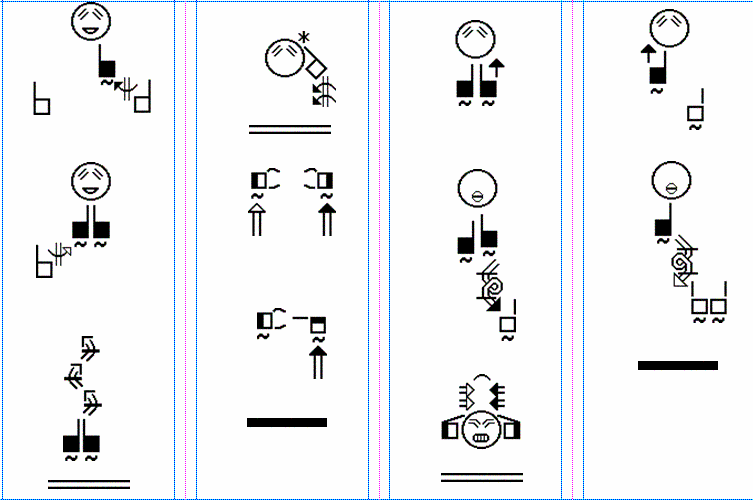
\includegraphics[width=0.6\textwidth]{Graphics/arreglo_glifos_sutton.png}
    \caption{Ejemplo de una secuencia de glifos del sistema de escritura de señas \textit{Sutton SignWriting}. De manera vertical cada una de las cuatro secciones representa una seña}
    \label{fig:arreglo_glifos_sutton}
\end{figure}
 
 Dado que \textit{SignWriting} representa la formación física real de los signos en lugar de su significado [Fig \ref{fig:arreglo_glifos_sutton}], no se requiere ningún análisis fonético o semántico de un idioma para escribirlo. Una persona que ha aprendido el sistema puede ``sentir'' un signo desconocido de la misma manera que una persona que habla inglés puede ``pronunciar'' una palabra desconocida escrita en el alfabeto latino, sin siquiera saber qué significa el signo.\brackcite{signwriting}

Las palabras pueden estar escritas desde el punto de vista del firmante o del espectador. Sin embargo, casi todas las publicaciones utilizan el punto de vista del firmante y asumen que la mano derecha es dominante. Existen varios símbolos de puntuación que corresponden a comas, puntos, signos de interrogación y exclamación y otros símbolos de puntuación de otras escrituras. Estos se escriben entre signos, y las líneas no se rompen entre un signo y su siguiente símbolo de puntuación.

La escritura de seña facilita enormemente la estandarización de las lenguas de señas, pero, a pesar de ello, no se encuentra popularizada globalmente y no se tiene constancia, al momento del autor realizar este trabajo, de que sea empleada en Cuba, por lo que otras alternativas como el reconocimiento de lenguas de señas pudieran ser de más utilidad.

\section{Reconocimiento de la Lengua de Señas}\label{section:state-of-the-art:slr}
El reconocimiento de la lengua de señas es ampliamente usado en diversos proyectos actualmente \brackcite{camgoz2020sign}. Se emplea en la identificación de gestos usando conjuntos de datos existentes
previamente. Las dos manos, la cabeza, los ojos, los
labios y el cuerpo  son, en esencia, lo utilizado en las lenguas de señas para realizar infinidad de gestos dedicados a funciones lingüísticas \brackcite{sandler2012dedicated}. Al ser los gestos una parte fundamental de este tipo de lenguas, se requiere de su reconocimiento específico. Los métodos de reconocimiento de gestos se pueden dividir en dos grandes grupos, en dependencia si utilizan un enfoque basado en hardware como Kinect u otros tipos de sensores, o un enfoque basado en software \brackcite{mitra2007gesture}. Dentro de este segundo enfoque destaca la detección de gestos por MediaPipe Holistic de Google, logrando muy buenos resultados en dichas tareas \brackcite{mediapipe_2020} [Fig \ref{fig:mediapipe}] .


\begin{figure}[ht!]
    \centering
    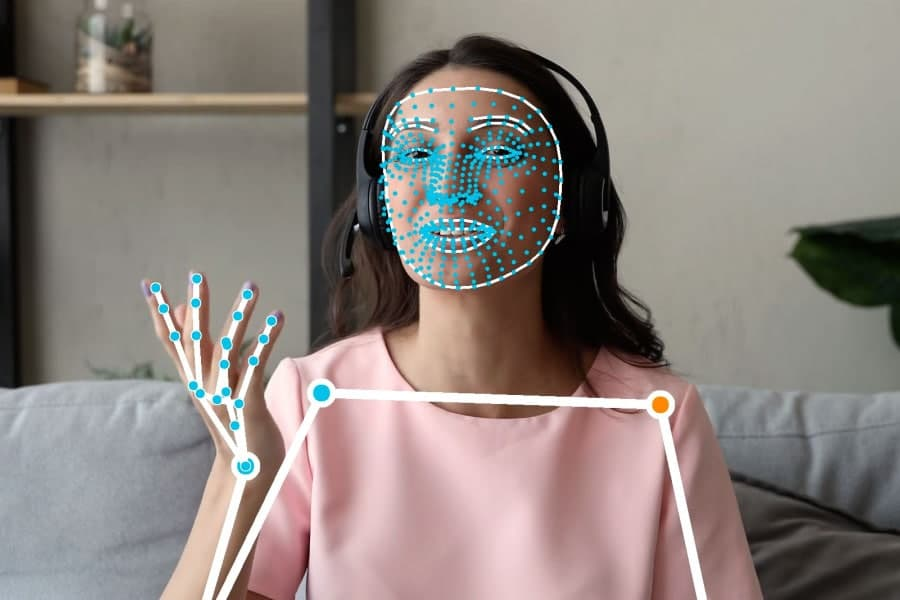
\includegraphics[width=0.6\textwidth]{Graphics/mediapipe.png}
    \caption{Software MediaPipe Holistic de Google, ejecutando un reconocimiento sobre una mujer.}
    \label{fig:mediapipe}
\end{figure}

Las diferentes vías de reconocimiento de señas aportan información valiosa para la comprensión cinética, estructural y lingüística de cada lengua de señas. Esto ayuda en la comprensión en un sentido, del oyente hacia el hipoacúsico, ya que este último es entendido por el oyente pero no en el otro sentido. Es por ello que se hace necesario el uso de formas de reforzar el entendimiento de la persona sorda hacia el oyente.

\section{Tecnología de avatares}\label{section:state-of-the-art:avatars}

La traducción automática de lenguas de señas, aplicando la tecnología de generación de avatares, ha sido empleada en proyectos como ViSiCAST  y eSIGN [véase Fig \ref{fig:avatares-visicast}], apoyados por la Unión Europea \brackcite{visicast_at_uea_2021} \brackcite{esign_at_uea_2021}. Se utilizan para traducir de las lenguas habladas a las lenguas de señas, lo cual solamente concierne la parte del avatar en sí. Las animaciones para las señas individuales son generadas basándose en las señas no manuales de datos complementarios y en señas individuales. Los procesos para generar los avatares incluyen una serie de pasos bastante complejos.
 
\begin{figure}[ht!]
    \centering
    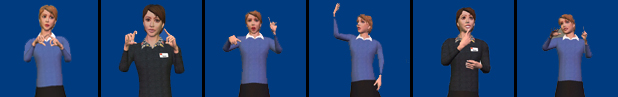
\includegraphics[width=0.6\textwidth]{Graphics/avatares_visicast.png}
    \caption{Muestra de los avatares de ViSiCAST, efectuando algunos movimientos}
    \label{fig:avatares-visicast}
\end{figure}

 
Los aspectos referentes a la velocidad, el ritmo y el tamaño deben ser tomados en
consideración utilizando reglas para controlarlos, ser configurados por un humano o
como resultado de un modelo de aprendizaje de máquina \brackcite{Nguyen2021AutomaticGO}. Otro de los usos que tienen estos métodos es lograr el anonimato en los videos y, cabe remarcar, que  son relativamente nuevos comparándolos con otros métodos de traducción automática de lenguas de señas \brackcite{kang2010effect} \brackcite{saragih2011real}.

Uno de los más grandes desafíos es que los avatares luzcan como humanos. En diversos estudios se comparan los gestos de los avatares con los gestos de los
humanos incluyendo algunos trabajos que han obtenido buenos resultados en Reino Unido en cuanto a generar dichos avatares con rasgos humanos utilizando modelos generativos \brackcite{stoll2018sign}. En Corea, usando el mismo corpus del trabajo anterior, se han logrado avances en un enfoque no auto-regresivo para lograr resultados incluso mejores \brackcite{hwang2021non}.

 Entre las tecnologías más utilizadas para la generación de avatares por animación se encuentran:
 \begin{itemize}
 \item  Unity
 \item Unreal 4
 \item Blender
 \item Maya3D 
 \item DirectX
 \end{itemize}  
 
 Se han desarrollado lenguajes de marcado para automatizar la generación de avatares de una forma dinámica y flexible \brackcite{latoschik2017effect} \brackcite{aneja2019high}. El estado del arte en la generación de avatares no está completamente automatizado, la mayoría de las partes del proceso de generación incluyen intervención humana para lograr buenos resultados. Gran parte de las investigaciones miden la calidad de las animaciones de avatares de forma perceptual y de estudios comprensivos con participantes sordos-mudos, incluyendo investigaciones metodológicas y recursos compartidos \brackcite{huenerfauth2006generating} \brackcite{kacorri2017regression}.
 
 En cuanto a la generación automática de avatares, han ocurrido recientes avances al poderse utilizar una interfaz de programación de aplicación de uno de los motores gráficos mencionados anteriormente. Se utilizan como medio para enlazar un archivo de captura de movimiento a una armadura predefinida en el motor gráfico, como por ejemplo una jerarquía de visión biótica (BVH, por sus siglas en inglés) a un diseño 3D de una persona \brackcite{Nguyen2021AutomaticGO}. Aún así, estas señas aisladas no son capaces de generar todo el vocabulario posible de la lengua de señas específica, por lo que convendría poseer una manera de crear cualquier secuencia de señas, dado un vocabulario establecido, mediante algún tipo de interpolación entre ellas.

\section{Modelos Generativos}
Durante la última década se ha visto un marcado incremento en lo que vienen siendo programas capaces de generar imágenes con un alto nivel de realismo, pero sin copiar nada de ninguna otra parte, siendo  ``auténticas'' de cierta forma. Esto es gracias a los denominados modelos generativos. Una nueva generación de modelos de redes neuronales capaces de aprender a hacer imágenes desde cero.\\

\subsection{Redes Generativas Adversariales}

Las Redes Generativas Adversariales (GANs) han logrado resultados impresionantes en varias tareas de síntesis de imágenes, y se están convirtiendo en un tema popular en la investigación de la visión por computadoras, debido al impresionante rendimiento que han alcanzado en diversas aplicaciones. Este modelo se ha impuesto desde que Goodfellow\brackcite{goodfellow2020generative} lo propuso en 2014.
Las GANs consisten en un generador G que se utiliza para generar muestras realistas a partir de ruido aleatorio e intenta engañar al discriminador D. El discriminador D se utiliza para identificar si la muestra es real o generada por G. El generador y el discriminador compiten entre sí hasta que el discriminador no puede distinguir entre las imágenes reales y las falsas [Fig \ref{fig:gan-design}].

\begin{figure}[ht!]
    \centering
    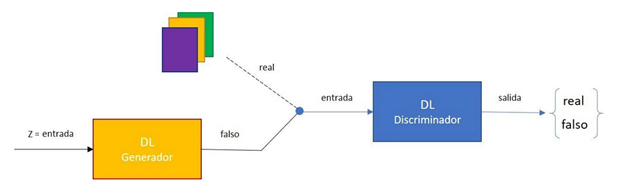
\includegraphics[width=0.6\textwidth]{Graphics/gan-design.png}
    \caption{Diseño de la arquitectura de redes adversariales generativas. En amarillo con una G se identifica al generador, mientras que el discriminante se identifica con el color azul y una D en el nombre. Arriba se puede apreciar la entrada de datos.}
    \label{fig:gan-design}
\end{figure}

\subsection{Redes Generativas Adversariales Condicionales}
Las GANs condicionales (CGAN) consisten en un Generador y Discriminador condicionados durante el entrenamiento mediante el uso de alguna información adicional [Fig \ref{fig:cgan-design}]. Esta información auxiliar podría ser, en teoría, cualquier cosa, como una etiqueta de clase, un conjunto de etiquetas o incluso una descripción escrita \brackcite{langr2019gans}. 
Durante el entrenamiento de CGAN, el Generador aprende a producir ejemplos realistas para cada etiqueta o descripción en el conjunto de datos de entrenamiento, y el Discriminador aprende a distinguir los pares ejemplo-etiqueta falsos de los pares ejemplo-etiqueta reales. \brackcite{langr2019gans}
Por lo tanto, para engañar al discriminador, no basta con que el generador de CGAN produzca datos de aspecto realista. Los ejemplos que genera también deben coincidir con sus etiquetas. Una vez que el Generador está completamente entrenado, nos permite especificar qué ejemplo queremos que sintetice el CGAN pasándole la etiqueta deseada.\brackcite{langr2019gans}

\begin{figure}[ht!]
    \centering
    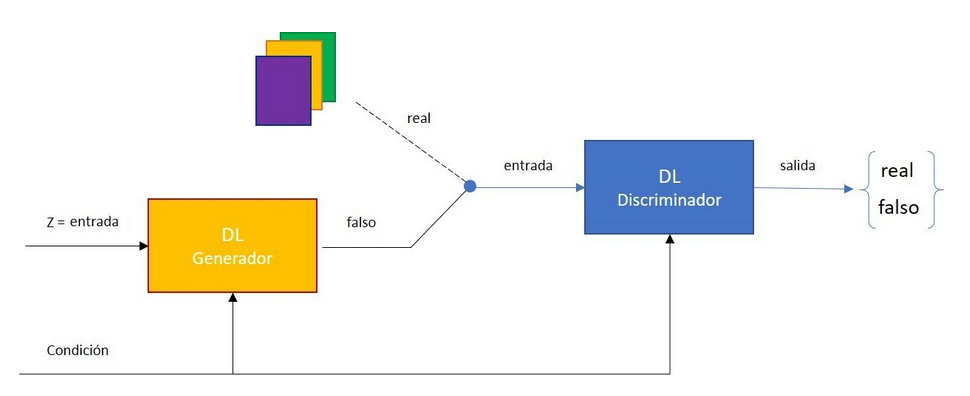
\includegraphics[width=0.6\textwidth]{Graphics/cgan-design.png}
    \caption{Diseño de la arquitectura de redes adversariales generativas condicionales. En amarillo con una G se identifica al generador, mientras que el discriminante se identifica con el color azul y una D en el nombre. Abajo de ellos se puede apreciar la entrada de datos}
    \label{fig:cgan-design}
\end{figure}

\subsection{Imágenes a partir de imágenes}
La traducción de imagen a imagen mediante redes generativas adversariales ha suscitado una gran atención en la investigación sobre el aprendizaje supervisado y no supervisado. Las GAN de ruido a imagen generan imágenes realistas a partir de muestras aleatorias de ruido, mientras que las GAN de imagen a imagen generan imágenes diversas a partir de imágenes. Se han propuesto muchas variantes de GAN, que han logrado buenos resultados en este tipo de tareas de traducción.
El objetivo de la traducción de imágenes es aprender el mapeo del dominio de la imagen de origen al de la imagen de destino, cambiando el estilo o algunas otras propiedades mientras mantiene el contenido de la imagen\brackcite{wang2020state}.
\subsubsection{Texto a imágenes}
En esta formulación, en lugar de utilizar ruido u otra imagen como entrada para el Generador, se utiliza una descripción textual de lo que se desea generar. Dicho texto es transformado primero en una incrustación (\textit{embedding}) de texto, el cual se concatena con el vector de la imagen a generar y luego se da como entrada al Generador.  Esta formulación ayudará al Generador a crear imágenes alineadas con la descripción de entrada en lugar de generar imágenes aleatorias\brackcite{wang2020state}.

\subsection{Otras formas de generación de imágenes}
Existen otras formas de generación de imágenes como el \textit{image inpainting}, la cual es una técnica de restaurar y reconstruir partes de una imagen basadas en la información de fondo de la misma. La edición de imágenes, la cual manipula principalmente las imágenes a través del color e interacciones geométricas para completar tareas como la deformación y la mezcla de imágenes. Otra forma es la síntesis de imágenes humanas, la cual tiene como objetivo manipular la apariencia visual de las imágenes de los personajes, transfiriendo la pose de un personaje a la pose objetivo, que puede calcularse a partir de otros personajes.\brackcite{wang2020state}

Además, en el último año, se ha visto un fuerte incremento de la adopción masiva de los modelos de difusión para la generación de imágenes, siendo Stable Difussion \brackcite{rombach2021highresolution}, un modelo de difusión latente, el que encabeza el podio, quedando segundos, Dall-E y Midjourney (otros modelos de difusión) [Fig \ref{fig:stable-diffusion}]. Este éxito de Stable Diffusion se debe a que, tanto los pesos, como el código, se encuentran disponibles públicamente, siendo además eficiente y menos exigente que sus otros competidores, permitiendo ejecutarlo y obtener buenos resultados en máquinas modestas con al menos 8Gb de VRAM.

\begin{figure}[ht!]
    \centering
    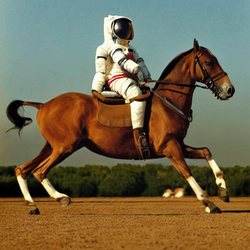
\includegraphics[width=0.6\textwidth]{Graphics/stable-diffusion.png}
    \caption{Imagen generada por Stable Diffusion}
    \label{fig:stable-diffusion}
\end{figure}

A pesar de, poder ser capaces de hacer más realistas los vídeos de forma aislada (a través del uso de img2img), sigue siendo necesaria encontrar la forma de concatenar de manera fluida varias señas. La forma usual de concatenación de varias imágenes, para obtener una calidad y fluidez realista en los videos generados, es a través de distintas técnicas de interpolación. Su uso en animaciones y generación de vídeo permite un resultado fluido y natural a la percepción de los usuarios y expectadores.

\section{Interpolación}\label{section:state-of-the-art:interpolation}
La interpolación es una forma de estimar datos nuevos en función de datos ya conocidos. Una técnica como esta puede ser aplicada para hacer predicciones en el campo de la economía y otras ramas. La dificultad con aplicarla en ese campo es la volatilidad del mismo que, sumado a los errores de precisión de la técnica, han llevado a los economistas a buscar otros métodos.\\

\subsection{Interpolación constante por partes}

El método de interpolación más simple es ubicar el valor de datos más cercano y asignar el mismo valor. En problemas simples, es poco probable que se use este método, ya que la interpolación lineal (ver a continuación) es más sencilla y devuelve mejores resultados con un menor número de puntos, pero en la interpolación multivariante de mayor dimensión, esta podría ser una opción favorable por su velocidad y simplicidad.


\subsection{Interpolación Lineal}
Una de las formas más simples es la interpolación lineal, la cual utiliza dos puntos ya conocidos $\left(x_{a}, y_{a} \right) $, $\left( x_{b}, y_{b}\right) $  y se usa la siguiente fórmula para estimar el punto $\left( x, y\right) $:
\begin{equation}
y = y_{a} + \left( y_{b} - y_{a}\right) \frac{x - x_{a}}{x_{b}-x_{a}}
\end{equation}
Esta ecuación anterior establece que la pendiente de la nueva recta entre $ \left(x_{a},y_{a}\right)$ y $\left(x ,y \right)$ es igual a la pendiente de la línea entre $\left(x_{a},y_{a}\right)$ y $\left(x_{b},y_{b}\right)$.\\

\subsection{Interpolación Cúbica}
Otra técnica de interpolación muy utilizada es la cúbica. Para utilizarla se necesita que la función $f\left( x \right) $ sea derivable y conocer los valores cuando $x=0$ y $x=1$, se utiliza un polinomio de grado tres y su derivada como se muestra a continuación:
\begin{align}
f\left( x \right) &= ax^3 + bx^2 + cx + d\\
f\prime\left( x \right) &= 3ax^2 + 2bx + c
\end{align}
Evaluando en los puntos $x=0$, $x=1$ y luego despejando se obtienen los siguientes valores:
\begin{align}
a &= 2f(0) - 2f(1) + f\prime(0) + f\prime(1)\\
b &= -3f(0) + 3f(1) - 2f\prime(0) - f\prime(1)\\
c &= f\prime(0)\\
d &= f(0)
\end{align}
Con eso se tiene todo lo necesario para la interpolación cúbica.\\
En caso de que no se conozca la derivada de la función,  se puede utilizar la derivada en puntos específicos. Si se tienen los puntos $\left(x_{0} ,p_{0} \right)$, $\left(x_{1} ,p_{1} \right)$,$\left(x_{2} ,p_{2} \right)$,$\left(x_{3} ,p_{3} \right)$:
\begin{align}
f(0) &= p_1\\
f(1) &= p_2\\
f\prime(0) &= \dfrac{p_2 - p_0}{2}\\
f\prime(1) &= \dfrac{p_3 - p_1}{2}
\end{align}
Combinando estos valores con la fórmula de la interpolación cúbica se obtiene:
\begin{align}
a &= -\tfrac{1}{2}p_0 + \tfrac{3}{2}p_1 - \tfrac{3}{2}p_2 + \tfrac{1}{2}p_3\\
b &= p_0 - \tfrac{5}{2}p_1 + 2p_2 - \tfrac{1}{2}p_3\\
c &= -\tfrac{1}{2}p_0 + \tfrac{1}{2}p_2\\
d &= p_1
\end{align}
Por lo que la fórmula de interpolación queda:
\begin{equation}
\begin{split}
f(p_0,p_1,p_2,p_3,x) &= (-\tfrac{1}{2}p_0 + \tfrac{3}{2}p_1 - \tfrac{3}{2}p_2 + \tfrac{1}{2}p_3)x^3 + \\ 
& (p_0 - \tfrac{5}{2}p_1 + 2p_2 - \tfrac{1}{2}p_3)x^2 + (-\tfrac{1}{2}p_0 + \tfrac{1}{2}p_2)x + p_1
\end{split}
\end{equation}
Esta forma de interpolar se conoce como Catmull-Rom spline.

\subsection{Otros métodos de interpolación}
Entre otros métodos que quedan sin comentar se encuentran:
\begin{itemize}

\item \textbf{La interpolación polinomial} la cual no es más que una generalización de la lineal y la cúbica.

\item \textbf{La interpolación por splines} que utiliza polinomios de bajo grado en cada uno de los intervalos y elige las piezas del polinomio de modo que encajen entre sí sin problemas. La función resultante es llamada spline.
 
\item \textbf{Interpolación mimética} la cual satisface las identidades del cálculo vectorial.

\end{itemize}

\subsection{Interpolación de movimiento}

La interpolación de movimiento (interpolación motriz) es una técnica de programación en la animación de personajes basada en datos que crea transiciones entre movimientos de ejemplo y extrapola nuevos movimientos.

Las acciones de ejemplo a menudo se crean a través de fotogramas clave o captura de movimiento. Sin embargo, la creación de fotogramas clave requiere mucha mano de obra y carece de variedades de movimiento, y ambos procesos dan como resultado movimientos que requieren mucho tiempo para modificarse. La interpolación motriz proporciona una alternativa mucho más rápida a la creación de nuevos movimientos a través de los mismos medios.\brackcite{Rose1998VerbsAA}


\section{Investigaciones y proyectos relacionados con la Lengua de Señas Cubana}\label{section:state-of-the-art:cubana}
En el área de las tecnologías de la información y las
comunicaciones sobre la Lengua de Señas Cubana  se pueden encontrar otros dos proyectos y/o trabajos.
 
 El desarrollo de una aplicación móvil [Fig. \ref{fig:app_cubana}] para dispositivos con sistema operativo Android, la cual esta enfocada en las familias con niños sordo-mudos, para brindarles el vocabulario necesario para interactuar con sus hijos \brackcite{android_app_lsc} y la tesis de grado referente al reconocimiento de la lengua de señas cubana usando métodos de traducción basados en inteligencia artificial y aprendizaje de máquina \brackcite{leynier-lsc-2021}.

\begin{figure}[ht!]
    \centering
    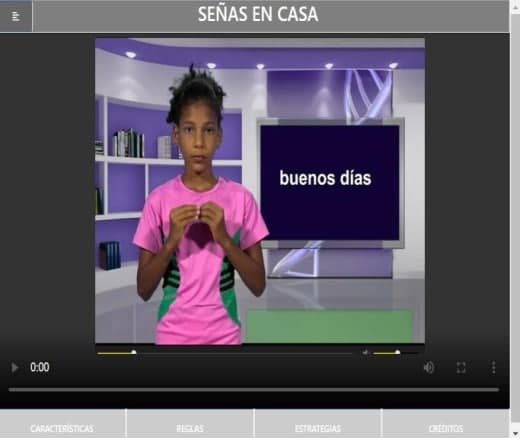
\includegraphics[width=0.6\textwidth]{Graphics/app_cubana.png}
    \caption{ Aplicación Android para la LSC \brackcite{android_app_lsc}}
    \label{fig:app_cubana}
\end{figure}

Se constata la existencia de una única investigación previa relacionada con la interpretación automática de la Lengua de Señas Cubana \brackcite{leynier-lsc-2021} pero ninguna en cuanto al tema que trata esta investigación.
\chapter{Propuesta}\label{chapter:proposal}
En esta sección se abordan los problemas principales presentados y la solución encontrada, para cada uno, en las respectivas secciones y se profundiza sobre nuevos problemas hallados, los cuales fueron resueltos para un mejor efecto final. Por otra parte, se proponen formas de facilitar la utilización e inter-operabilidad de la propuesta presentada. 

%%%%%%%%%%%%%%%%%%%%%%%%%%%%
% MOSTRAR FOTO DE CADA PROBLEMA
%%%%%%%%%%%%%%%%%%%%%%%%%%%%

\begin{figure}[ht!]
\centering
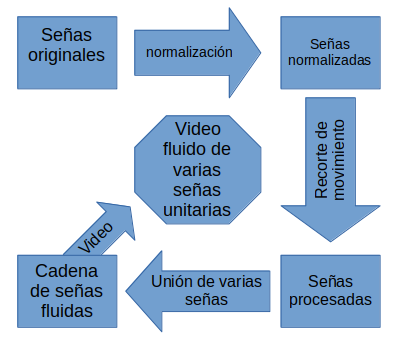
\includegraphics[width=0.5\textwidth]{./Graphics/esquema}
\caption{Esquema del enfoque a utilizar}
\label{f:enfoque_esquema}
\end{figure}

Se utilizara un enfoque basado en la interpolación de movimiento para lograr la correcta concatenación y fluidez para la generación gráfica de señas. Dado un conjunto de señas unitarias se deberá efectuar un correcto procesamiento de las mismas y lograr unir varias de ellas en un video de manera fluida, haciendo así posible la generación de señas [véase Fig \ref{f:enfoque_esquema}]. 



\section{Definiciones}

Se define como un video $V$ a la secuencia de puntos extraídos. $V_i$
constituye el i-ésimo cuadro (\emph{frame}) del video. Un frame $F$ está compuesto por una secuencia
de puntos en el espacio, representando las posiciones de las diferentes partes del cuerpo extraídas,
$F_i$ representa el i-ésimo punto del frame y $F_{parte}$ representa los puntos asociados a la parte 
descrita en el frame. 

\subsection{Operaciones vectoriales}

Las operaciones vectoriales constituye operaciones realizadas sobre los vectores. Estas operaciones 
pueden representar diferentes acciones a un nivel de abstracción mayor sobre los vectores. Sean $a$ y
$b$ vectores o puntos de tres dimensiones entonces:

\begin{itemize}
	\item $a - b$: Representa el vector de la dirección del punto $b$ hacia $a$.
	\item $a + b$: Representa la traslación del punto $a$ ($b$) en dirección $b$ ($a$).
	\item $a \times b$: Representa un vector perpendicular a $a$ y $b$.
	\item $\cos \theta = \frac{a \cdot b}{||a|| \cdot ||b||}$: Representa el coseno del ángulo $\theta$
	entre los vectores $a$ y $b$.
	\item $\alpha a$: Representa el vector siendo escalado por un factor $\alpha$.
\end{itemize}

\subsubsection{Rotación de Rodríguez}

La rotación constituye en girar sobre un eje $k$ un vector $v$, $\theta$ grados, donde ambos vectores son 
unitarios. Este vector rotado puede ser hallado mediante:
$$
rotación(v, k, \theta) = v \cos \theta + (k \times v) \sin \theta + k(k \cdot v)(1 - \cos \theta)
$$.


\section{Preprocesamiento de los datos}
Al utilizar datos por primera vez siempre es una buena práctica analizarlos y reconocer la estructura que poseen. La gran mayoría de las veces los datos con los que se trabaja vienen originalmente con fallas estructurales o de valores que no pertenecen al dominio que se trabaja. Es por este motivo que se hace fundamental, siempre que se vaya a realizar un trabajo con datos, realizarle su correspondiente análisis estructural y detectar posibles errores que se contengan en los mismos.
\subsection{Obteniendo el conjunto de datos}
De anteriores investigaciones contamos con un corpus de señas unitarias las cuales tienen la siguiente estructura :
$$
(r,f,p,c)
$$
 
donde :
\begin{itemize}
 \item $r$ indica la representación a la que se accede de dicha frase nominal en el conjunto de datos.
 \item $f$ refiere al frame al que se accede de dicha representación
 \item $p$ representa el punto al que se indexa de dicho frame
 \item $c$ indica la componente del punto a la que se accede
\end{itemize}
 
  Una seña unitaria no es más que una secuencia que representa a una frase nominal, dígase como ejemplo la seña que significa  ``américa del sur''. 

\subsection{Limitando a una sola seña por frase}
Luego de tener el conjunto de frases curadas y limpias, quedaba aún el problema de las palabras repetidas que tienen más de una seña, en dependencia de qué léxico del corpus brindado por el CENDSOR se revise.
Para dicho problema se optó por escoger solamente la primera que apareciera, puesto que solo complejizaría más la tarea presentada dado que, para una misma frase en el corpus, podía incurrir en una variación bastante considerable, es decir, la señas para una misma palabra de un intérprete a otro variaban mucho para el caso de la palabra ``paz'' con 4 tipos de señas distintas (como si de una ``falta de ortografía'' se tratase). 

\subsection{Detección de problemas}
A pesar de que todos los videos poseen una estructura similar, manteniéndose un fondo fijo de un color constante, los señantes presentes en los mismos son distintos unos de otros, así como también sus movimientos realizados. Aun refiriéndose a la misma seña, las diferencias no dejaban de aparecer, tanto en estructura corporal, como en velocidad y variaciones de la seña.

En algunos casos, los videos presentaban una secuencia de imágenes sin señante inicialmente, lo que generaba que el modelo dedicado al reconocimiento corporal fallara en dicha tarea, devolviendo un conjunto de ceros, en esos cuadros (frames). Algo similar, ocurría cuando no se detectaban bien las manos del intérprete (ya sea por salirse de la ventana de enfoque de la cámara o encontrarse de forma perpendicular a la misma), haciendo que estas no aparezcan en algún que otro frame.

Para el primer caso la solución fue, sencillamente, no tomar en cuenta los frames que todos sus puntos fueran nulos; mientras que el segundo caso no era tan trivial puesto que, a pesar de no tener las manos, el cuerpo si se detecta y proporciona información importante del movimiento del señante por lo que se decidió dejar dichos conjuntos para una posterior revisión.

\subsubsection{Análisis preliminar de los datos}

Al analizar los datos se encontraron varios problemas:
\begin{itemize}
	\item Los puntos asociados a las manos no se encontraban sobre las muñecas.
	\item Los puntos de las manos no existían en intervalos del video.
	\item El tamaño del señante varía entre videos.
	\item El video contiene frames en los cuales no se realiza ningún movimiento.
\end{itemize}

\subsection{Limpieza de los datos}

 A todas las palabras se le hace limpieza con expresiones regulares para eliminar la mayoría de imperfecciones posibles en las palabras, el uso de ``nn'' en lugar de la ``ñ '' y la presencia de números puesto que al agrupar las frases de varios léxicos distintos, estos se renombraban. Este procesamiento de las palabras es de utilidad para conformar el dataset lo más preciso posible, evitando la repetición de las frases.
 
\subsubsection{Arreglando errores ortográficos}

Durante la creación del conjunto de datos se detectaron, además, frases nominales inexistentes y/o con errores ortográficos, corrigiéndose una pequeña cantidad de estas a mano con un diccionario de palabras, dado que la gran mayoría de los errores ortográficos eran tildes ausentadas.

\section{Problema de la visualización de los datos}
Los datos ya procesados, del trabajo de Gutiérrez-González \brackcite{leynier-lsc-2021}, son solamente arreglos de dimensión (número de interpretaciones de la seña, (número de frames de la seña,  número total de puntos * 3)), lo cual no facilita  interpretar o detectar posibles problemas. Para solventarlo se recurrió a graficar los puntos en un espacio tridimensional. Se realizaron las transformaciones pertinentes (rotación por el eje z y usando un grado de elevación de 90 grados)  para que se visualizara de frente al espectador, permitiendo, al tener guardada información de las uniones, la visualización de líneas entre dichos puntos espaciales.

\begin{figure}[ht!]
    \centering
    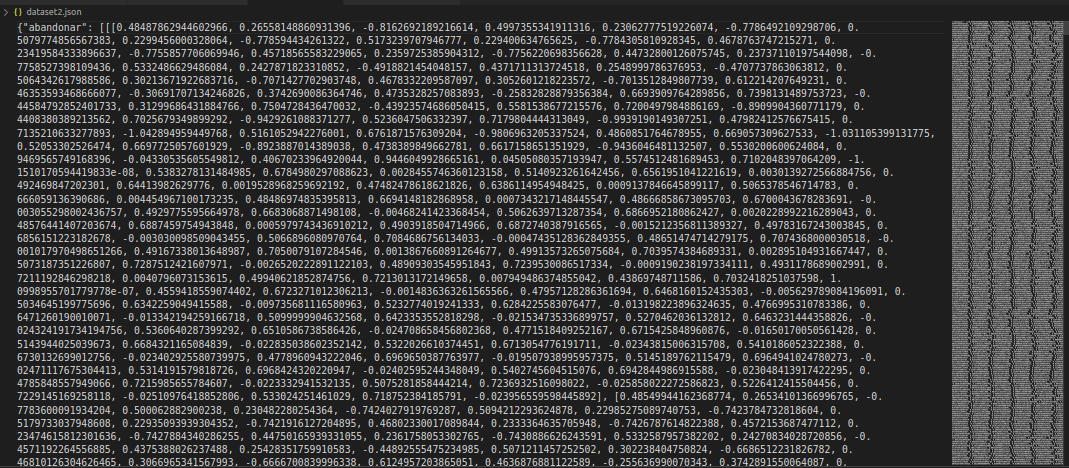
\includegraphics[width=0.6\textwidth]{Graphics/data_example.png}
    \caption{Ejemplo parcial de la representación de los datos dentro de uno de los conjuntos de datos. Se puede apreciar la frase nominal ``abandonar' seguida de parte de su representación'}
    \label{fig:data_example}
\end{figure}


Se utilizan solamente los puntos del cuerpo y de las manos obtenidos a través de la investigación antes mencionada. Se constan de 67 puntos espaciales siendo 25 del cuerpo y la cabeza (obviando el tren inferior de puntos), 21 para la mano derecha e ídem para la mano izquierda [Fig \ref{fig:points}]. 

\begin{figure}[ht!]
    \centering
    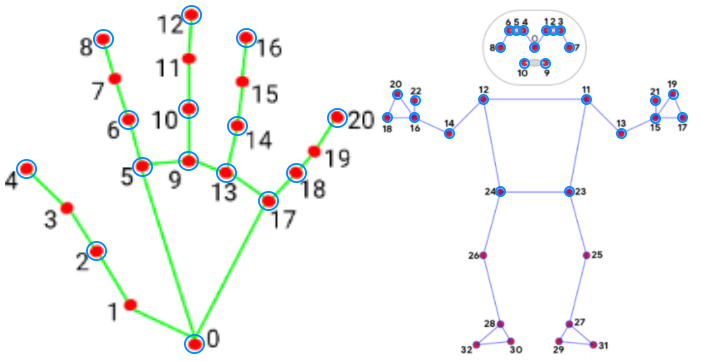
\includegraphics[width=0.6\textwidth]{Graphics/points.png}
    \caption{Algunos de los puntos que extrae Mediapipe Holistic. De izquierda a derecha apreciamos los puntos de la mano derecha y los puntos del cuerpo.}
    \label{fig:points}
\end{figure}

\section{Problema de manos que no se encontraban sobre las muñecas}

Las manos en los datos se encuentran definidas como una secuencia de puntos $F_{mano\_izquierda}$ y 
$F_{mano\_derecha}$, en ambos casos el primer punto de cada una representa el punto asociado a la muñeca 
en la mano. A su vez el cuerpo posee otra representación de la muñeca $F_{muñeca\_cuerpo\_izquierda}$ y $F_{muñeca\_cuerpo\_derecha}$. 
Estos puntos en los datos deberían
estar juntos o relativamente cercanos, sin embargo, en los datos se encontraban a una distancia considerable.

Para la solución del problema se calcula el vector dirección entre las representaciones de las muñecas del cuerpo 
y las muñecas de las manos y se trasladan los puntos de las manos en esta dirección, dejando ambas muñecas en el 
mismo sitio.

\begin{align}
d &= F_{muñeca\_cuerpo\_izquierda} - F_{muñeca\_mano\_izquierda} \\
F_{mano\_izquierda}' &= F_{mano\_izquierda} + d
\end{align}

\section{Problema de las manos faltantes}

Este problema consiste en que en ciertas secciones del video los puntos asociados a las manos fallan al ser 
encontrados por los modelos de reconocimiento [véase Fig \ref{f:manos_faltantes}]. Este problema se divide en dos casos:

\begin{itemize}
\item Faltan en los frames internos de la seña [véase Fig \ref{f:manos_faltantes}]
\item Faltan las manos en los frames extremos de la seña [véase Fig \ref{f:fluidez_variable}]
\end{itemize}

\begin{figure}[t]
	\begin{subfigure}[t]{0.3\textwidth}
	\centering
		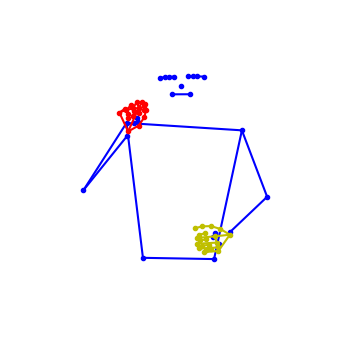
\includegraphics[align=t,width=0.9\linewidth, height =0.9\linewidth]{Graphics/mano_antes_desaparecer.png}
		\caption{Mano antes de desaparecer del token ``aborto''}
		\label{f:mano_antes_desaparecer}
	\end{subfigure}
	\begin{subfigure}[t]{0.3\textwidth}
	\centering
		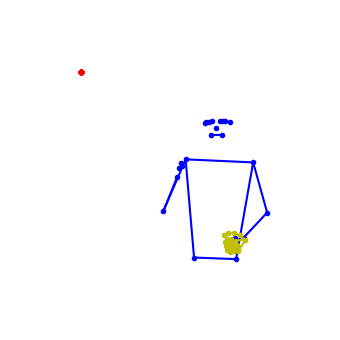
\includegraphics[align=t,width=0.9\linewidth, height =0.9\linewidth]{Graphics/mano_desaparecida.png}
		\caption{Mano derecha desaparecida del mismo token al siguiente frame }
		\label{f:mano_derecha_desaparecida}
	\end{subfigure}
		\begin{subfigure}[t]{0.3\textwidth}
	\centering
		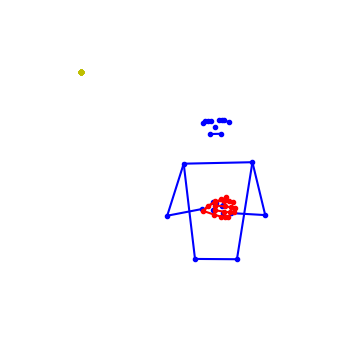
\includegraphics[align=t,width=0.9\linewidth, height =0.9\linewidth]{Graphics/mano_faltante_interna.png}
		\caption{Mano izquierda desaparecida del mismo token en otro frame distinto}
		\label{f:mano_izquierda_desaparecida}
	\end{subfigure}
	\caption{Ejemplo del segundo caso de  manos faltantes.}
	\label{f:manos_faltantes}
\end{figure}

\subsection{Frames internos}
La solución propuesta para el primer caso es interpolar las posiciones intermedias faltantes teniendo como 
partida los últimos puntos existentes de las manos antes de desaparecer y como llegada los primeros puntos existentes 
luego de la desaparición. Para esto se define el operador interpolación $I$, el cual toma dos conjuntos de puntos, los 
puntos de partida y los de llegada, y un número representando la cantidad de elementos a devolver uniformemente
escogidos en el intervalo a interpolar. El resultado de aplicar 
$I(V[i]_{mano\_izquierda}, V[i + k]_{mano\_izquierda}, k - 1)$ es el conjunto interpolado de $k-1$ frames 
entre los frames $i$ e $i+k$. Al aplicar este método en cada intervalo en los cuales no estaba definida las manos 
se llenan estos huecos.
\subsection{Frames extremos}
En el segundo caso no se puede realizar la interpolación, debido a que no existe un conjunto de llegada o de partida. Al probar con distintos conjuntos de señas, resaltó el hecho de que las señas que comenzaban sin manos, durante un largo período de tiempo, causaban errores y fallos en la solución de la sección \ref{section:proposal:fluidez}.  Por lo que la forma de resolver dicho inconveniente devino del uso de una mano falsa, como si de una prótesis se tratara, la cual se compone del mismo número de puntos de una mano real y la misma fue situada gracias a que el cuerpo contiene puntos coincidentes para este mismo propósito.

Para resolver el problema se creó una mano en posición semi-extendida para que actuara de prótesis en los lugares 
donde ocurre el problema. Esta mano prótesis necesita ser modificada para que se pueda colocar en el lugar correcto 
en cuerpo. En primer lugar se realiza una rotación de esta de tal forma que quede alineada con el brazo, luego dicha 
mano es trasladada hacia la muñeca del cuerpo.

Se realizaron transformaciones espaciales, rotaciones y se seleccionaron matrices específicas para operar con los puntos de la mano falsa y así obtener su homologa contraria, además de permitir ajustarla al plano regido por el codo, la muñeca y los tres puntos coincidentes. Todo este conjunto de operaciones, sumado al hecho de utilizar la proporción de cuanto mide el antebrazo respecto a la medida desde la muñeca y la base del dedo medio, permitieron el correcto estiramiento y adaptación de la mano falsa a las distintas estructuras corporales evidenciadas en el conjunto de datos.

\begin{align}
\begin{split}
brazo\_izq &= normalizar(F_{muñeca\_cuerpo\_izquierdo} - ... \\
& F_{codo\_izquierdo})
\end{split}\\
\begin{split}
muñeca\_izq\_dirección &= normalizar(F_{muñeca\_mano\_izquierda} - ... \\
& F_{nudillo\_dedo\_medio\_izquierdo})
\end{split}\\
eje\_rotación &= normalizar(brazo_izq \times muñeca\_izq\_dirección) \\
ángulo &= \arccos brazo\_izq \cdot muñeca\_izq\_dirección \\
F_{mano\_izquierda} &= rotación(F_{mano\_izquierda}, eje\_rotación, ángulo) \\
d &= F_{muñeca\_cuerpo\_izquierda} - F_{muñeca\_mano\_izquierda} \\
F_{mano\_izquierda} &= F_{mano\_izquierda} + d
\end{align}

\section{Problema de la fluidez en la unión de varias señas}\label{section:proposal:fluidez}
La fluidez en la generación de avatares es de vital importancia, puesto que una de las metas es lograr la mayor semejanza posible al movimiento natural de una persona. Al pensar en concatenar dos señas lo primero que se imagina es un movimiento suave y que se logren identificar ambas secuencias, cosa que no ocurre al unir dos secuencias sin ningún tipo de procesamiento como los videos con que se cuentan. No todos los intérpretes terminaban la seña de la misma manera, ni en la misma posición [véase Fig \ref{f:fluidez_variable}], y en algunos casos hasta ocurrían periodos largos de inactividad entre que terminaba la seña y el final del grabación. 


La solución encontrada a este problema fue interpolar entre ambas secuencias, obtando por la interpolación cúbica como candidata de mayor suavidad, si se requieren bastantes frames intermedios, y la lineal para casos de pocos frames o poca variación de movimiento.
Esta interpolación se realiza escogiendo una cantidad fija de puntos en dependencia del método escogido. Dichos puntos son separados por componentes y  se realiza la interpolación de forma individual en función de una lista de valores ``t'' asociados a cada una. Es decir, una lista t que enumera los valores de x es el argumento de la función a interpolar, dejándose por medio los valores asociados a la cantidad a interpolar, mientras que los valores obtenidos en la lista x serían los valores de la evaluación de dicha función en los valores de t conocidos.

\subsection{Frames variables intermedios}
Durante la concatenación también existe un diferencial de movimiento entre el final de una seña y el inicio de otra. El problema aquí es 
que existen poses que terminan más distantes de su continuación que otras, haciendo que 
la transición sea o muy rápida o muy lenta, por esto se decide hacer una transición con frames
variables en dependencia de la diferencia. Algunos de los videos terminan reposando ambas manos superpuestas sobre el vientre, mientras que en otros se termina descansando los brazos paralelamente al cuerpo o terminan de cualquier otra forma. Además, la distancia del señante a la cámara es, también, muy variable, por lo que se denota como movimiento dada la diferencia de posición.

\subsection{Unión de señas}

La unión de señas constituye la operación de unir dos señas para conformar una sola. Esta operación
es realizada mediante el operador de interpolación al unir los videos $V_1$ y $V_2$, una vez realizadas todas 
las operaciones anteriores, de la siguiente forma:

\begin{equation}
V = I(V_1[n], V_2[0], frames\_de\_intercambio)
\end{equation}

Se observa que hace falta conocer la cantidad de $frames\_de\_intercambio$, este valor debe depender de la diferencia
entre $V_1[n]$ y $V_2[0]$ ya que vectores parecidos deben de tener menos frames de transición que vectores más distantes [véase Fig \ref{f:fluidez_variable}).
Se define diferencia como la norma de la diferencia entre los vectores.

A criterio del autor se seleccionaron unos ejemplos en donde se sabía la variabilidad y la cantidad de frames buenas para el segmento a interpolar. Para obtener este valor se observaron varios valores de diferencia entre vectores y se decidió la cantidad de frames de 
intercambio para dicha diferencia [véase Tabla \ref{table:intercambio_frame}], con varias muestras se creó una función mediante interpolación de estos valores la cual 
permite conocer el valor de $frames\_de\_intercambio$ dada la diferencia.


\begin{table}[h!]
	\begin{center}
	  \caption{Valores a criterio del autor para interpolar según la variación de movimiento entre frames }
	  \label{table:intercambio_frame}
	  \begin{tabular}{c|c} 
		\textbf{Variación entre frames} & \textbf{Cantidad de frames}\\
		\hline
		0.0 & 1 \\
		0.5 & 7 \\
		4.6 & 14\\
	  \end{tabular}
	\end{center}
  \end{table}

\begin{figure}[t]
\centering
	\begin{subfigure}[t]{0.3\textwidth}
		\centering
		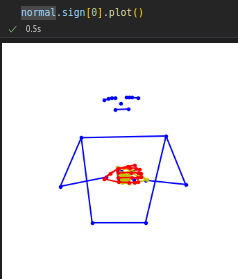
\includegraphics[align=t,width=0.9\linewidth, height =0.9\linewidth]{Graphics/principio_abandonar.png}
		\caption{Principio del token ``abandonar''}
		\label{f:principio_variable_abandonar}
	\end{subfigure}
		\begin{subfigure}[t]{0.3\textwidth}
		\centering
		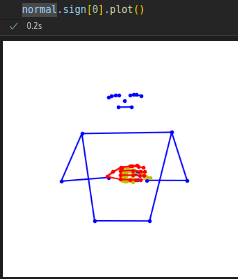
\includegraphics[align=t,width=0.9\linewidth, height =0.9\linewidth]{Graphics/principio_aborto.png}
		\caption{Principio del token ``aborto''}
		\label{f:principio_variable_aborto}
	\end{subfigure}
		\begin{subfigure}[t]{0.3\textwidth}
		\centering
		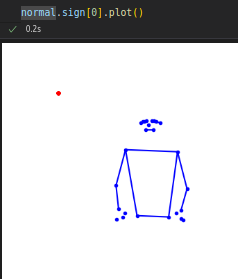
\includegraphics[align=t,width=0.9\linewidth, height =0.9\linewidth]{Graphics/principio_amar.png}
		\caption{Principio del token ``amar''}
		\label{f:principio_variable_amar}
	\end{subfigure}	
	\vskip 0pt
	\begin{subfigure}[t]{0.3\textwidth}
		\centering
		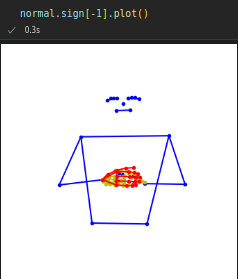
\includegraphics[align=t,width=0.9\linewidth, height =0.9\linewidth]{Graphics/final_abandonar.png}
		\caption{Final del token ``abandonar''}
		\label{f:final_variable_abandonar}
	\end{subfigure}
	\begin{subfigure}[t]{0.3\textwidth}
		\centering
		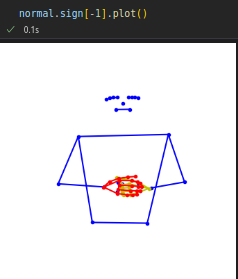
\includegraphics[align=t,width=0.9\linewidth, height =0.9\linewidth]{Graphics/final_aborto.png}
		\caption{Final del token ``aborto''}
		\label{f:final_variable_aborto}
	\end{subfigure}
	\begin{subfigure}[t]{0.3\textwidth}
		\centering
		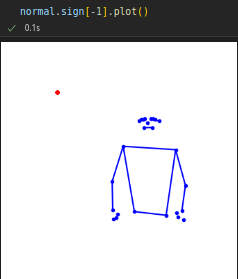
\includegraphics[align=t,width=0.9\linewidth, height =0.9\linewidth]{Graphics/final_amar.png}
		\caption{Final del token ``amar''}
		\label{f:final_variable_amar}
	\end{subfigure}
	
	\caption{Ejemplo de la diferencia entre extremos consecutivos de varios tokens, evidenciándose su variabilidad.}
	\label{f:fluidez_variable}
\end{figure}
El hecho de usar uno u otro método de interpolación, implica que se seleccionan distintas cantidades de puntos, como se explica en el estado del arte [véase sección \ref{section:state-of-the-art:interpolation}] . Siendo la más dinámica, con una menor cantidad de puntos, la interpolación lineal, pero, mínimo, se cuenta con 24 frames ya que equivalen a 1 segundo de un video de 24 fps(frames por segundo), lo cual es bastante estándar.


\subsection{Problema del tamaño del señante variable durante el video}

En los videos analizados se encuentran varios tipos de señante, estos tienen diferentes complexiones y también
se encuentran grabados desde diferentes distancias e inclinaciones. Esto trae como consecuencia que los puntos 
extraídos no tengan la misma configuración. Para esto se normalizan los puntos de cada frame $F$ teniendo como 
referencia la distancia entre los hombros. Esta distancia en cada frame es mantenido constante a un valor de $0.5$. Para lograr esto 
primero se calcula el factor de escalado del frame para que la distancia entre los hombros sea $0.5$ y luego este 
factor es aplicado a todos los puntos, logrando así una mayor homogeneidad entre los distintos señantes.

\begin{align}
factor\_de\_normalización &= \frac{0.5}{|| F_{hombro\_derecho} - F_{hombro\_izquierdo} ||} \\
F &= factor\_de\_normalización \cdot F
\end{align}

Con estas operaciones se mantiene una distancia constante de $0.5$ en cada frame.


\subsection{Inactividad en la secuencia}
Este problema surge debido a la naturaleza de los videos analizados. En estos el señante empieza y termina en una 
posición de descanso por lo que en esta etapa no ocurre un movimiento relativo a la seña descrita. Esto implica 
que al realizar la concatenación de videos aparecieran periodos con estas posiciones de descanso, lo cual impedía
una concatenación fluida. Esto no conlleva una solución tan trivial como simplemente recortar los frames con una cantidad fija, dado que cada video puede presentar anomalías que lo hagan parecer inactivo o pueden existir videos sin inactividad, con lo cual, al recortar, estaríamos eliminando parcialmente la seña. Para la solución de dicho problema se define una ecuación que mide el movimiento
en el video, luego nos quedamos con el intervalo de video que contenga la mayor parte del movimiento 
total del mismo y que tenga un intervalo lo más pequeño posible.

La ecuación de movimiento se define como:

\begin{equation}
mov(i) = || V[i+1] - V[i] ||
\end{equation}

Esta ecuación cuantifica el movimiento entre un frame y el próximo y por su definición es no negativa [véase Fig \ref{f:movediff_aborto_amar}], 
por lo tanto hallando su integral en el dominio se puede tener una medida del movimiento en el segmento.
Se defina la integral de $mov$ en el intervalo $i$, $j$ como:

\begin{equation}
integral\_mov(i,j)
\end{equation}

Se desea obtener un intervalo que contenga gran parte del movimiento pero que no sea el video completo, para esto 
se define el problema de optimización siguiente, donde $n$ es el frame final:

\begin{align}
\max_{i,j} &\frac{integral\_mov(i,j)}{j-i} \\
s.a: \qquad integral\_mov(i,j) &> integral\_mov(0,n) \cdot porciento\_de\_movimiento \\
& \qquad j > i
\end{align}

Obteniendo el intervalo que solucione el problema anterior se obtiene un nuevo video al quedarse solamente con los 
frames dentro de este intervalo, que aseguran que el movimiento en este es mayor al $porciento\_de\_movimiento$ seleccionado.
Dado que el problema es discreto la integral es calculada por métodos numéricos y el problema de optimización es 
resuelto probando los valores posibles de los intervalos $i,j$.

\begin{figure}[t]
	\begin{subfigure}[t]{0.3\textwidth}
	\centering
		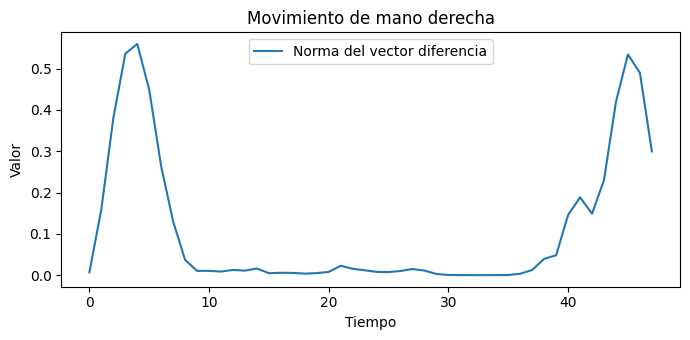
\includegraphics[align=t,width=0.9\linewidth, height =0.9\linewidth]{Graphics/amar_rhand_movediff_original_nu.png}
		\caption{Gráfica de movimiento de la mano derecha del token ``amar''}
		\label{f:rhand_movediff_amar}
	\end{subfigure}
	\begin{subfigure}[t]{0.3\textwidth}
	\centering
		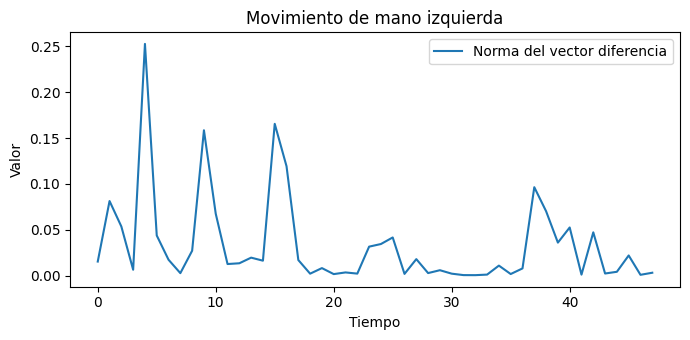
\includegraphics[align=t,width=0.9\linewidth, height =0.9\linewidth]{Graphics/amar_lhand_movediff_original_nu.png}
		\caption{Gráfica de movimiento de la mano izquierda del token ``amar'' }
		\label{f:lhand_movediff_amar}
	\end{subfigure}
		\begin{subfigure}[t]{0.3\textwidth}
	\centering
		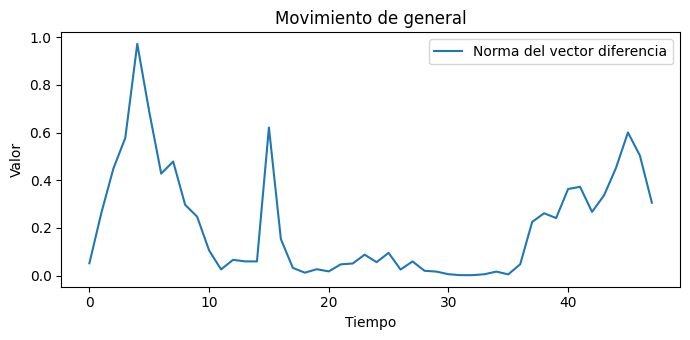
\includegraphics[align=t,width=0.9\linewidth, height =0.9\linewidth]{Graphics/amar_global_movediff_original_nu.png}
		\caption{Gráfica de movimiento general del token ``amar''}
		\label{f:general_movediff_amar}
	\end{subfigure}
	\vskip 0pt
	\begin{subfigure}[t]{0.3\textwidth}
	\centering
		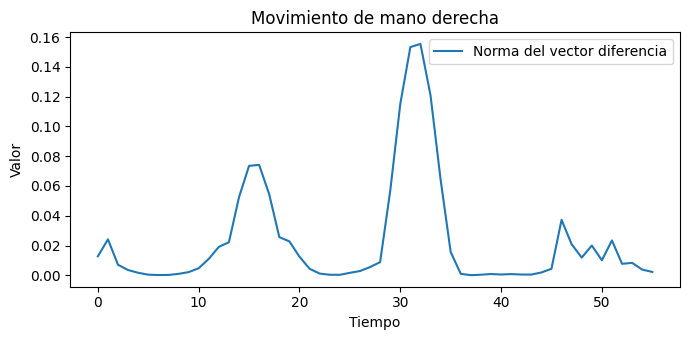
\includegraphics[align=t,width=0.9\linewidth, height =0.9\linewidth]{Graphics/aborto_rhand_movediff_original_nu.png}
		\caption{Gráfica de movimiento de la mano derecha del token ``aborto''}
		\label{f:rhand_movediff_aborto}
	\end{subfigure}
	\begin{subfigure}[t]{0.3\textwidth}
	\centering
		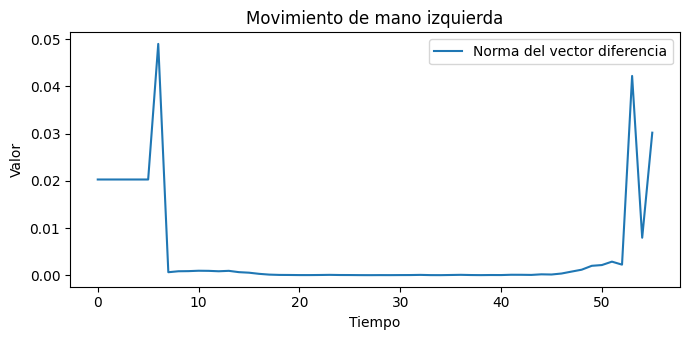
\includegraphics[align=t,width=0.9\linewidth, height=0.9\linewidth]{Graphics/aborto_lhand_movediff_original_nu.png}
		\caption{Gráfica de movimiento de la mano izquierda del token ``aborto''}
		\label{f:lhand_movediff_aborto}
	\end{subfigure}
	\begin{subfigure}[t]{0.3\textwidth}
	\centering
		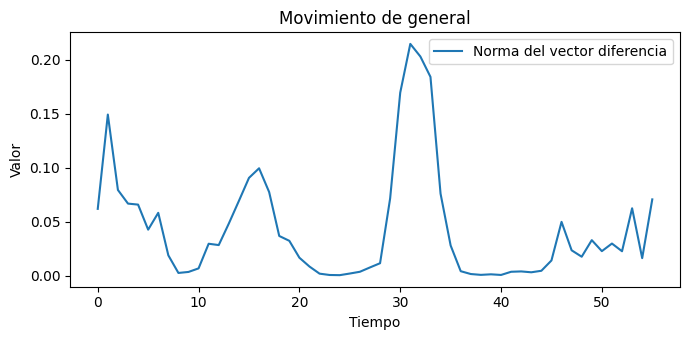
\includegraphics[align=t,width=0.9\linewidth, height=0.9\linewidth]{Graphics/aborto_global_movediff_original_nu.png}
		\caption{Gráfica de movimiento general del token ``aborto''}
		\label{f:general_movediff_aborto}
	\end{subfigure}
	\caption{Gráficas de movimiento por manos y general de los tokens ``amar'' y ``aborto''.}
	\label{f:movediff_aborto_amar}
\end{figure}


Resolver todos los problemas planteados anteriormente son fundamentales para la correcta generación de señas, puesto que, en caso de fallarse en solucionarse alguno de los problemas el resultado pudiera afectar negativamente la fluidez percibida por los usuarios, así como generar distorsiones durante la reproducción.
%%%%%%%%%%%%%%%%%%%%%%%
% POSIBLEMENTE PARA RECOMENDACIONES

\chapter{Detalles de Implementación y Experimentos}\label{chapter:implementation}
Para poder valorar la viabilidad de la propuesta realizada en este trabajo, es
necesaria la implementación de un prototipo del modelo explicado en el capítulo
anterior.

\section{Herramientas y tecnologías utilizadas}\label{section:implementation:techs}
\subsection{Lenguaje de programación Python}
Python es un lenguaje de programación de propósito general y alto nivel desarrollado por Guido van Rossum en 1991. Su filosofía de diseño enfatiza la legibilidad del código con el uso de sangría significativa. Python se tipifica dinámicamente y tiene incorporado un recolector de basura. Admite múltiples paradigmas de programación, incluida la programación estructurada, orientada a objetos y funcional. La más reciente  versión liberada al momento de realizarse este trabajo es la 3.11 [\cite{python_executive_summary_2022}].

Es altamente empleado para ingeniería y análisis de datos, aprendizaje de máquina
e inteligencia artificial gracias a sus infinidad de bibliotecas como NumPy, Tensorflow, Keras, Pytorch, SciPy, Pandas y Matplotlib, entre otras creadas tanto por el mismo equipo de trabajo de Python como la propia comunidad. Para desarrollo web cuenta con marcos de trabajo (frameworks) como Django. Es altamente utilizado en la educación al ser de fácil aprendizaje y asimilación logrando así reducir la barrera de entrada al mundo de la programación a todo aquel interesado.

 En la actualidad sigue manteniendo el primer puesto de los índices de TIOBE y PYPL ratificando el interés de gran parte de la población y de los empleadores por este lenguaje y las ventajas que ofrece. Grandes organizaciones como Google [\cite{quotes_about_python_2021}], el CERN [\cite{python_the_holy_grail_of_programming_2014}], la NASA [\cite{python_success_stories_2021}], Yahoo [\cite{organizationsusingpython}], Wikipedia, Amazon, Facebook, Instagram [\cite{meta_for_developers_2018}], Spotify, entre otros.
Para este trabajo se utilizó la versión 3.7 para lograr una retro-compatibilidad
alta.


\subsection{Numpy}
Constituye una biblioteca de Python de código abierto, la cual permite generar, tanto vectores como matrices, de grandes dimensiones y operar de manera cómoda y sencilla con ellos [\cite{numpy_2012}].
Consigue esto gracias a que utiliza internamente el lenguaje C para lograr efectuar de forma rápida operaciones muy costosas entre elevadas dimensiones.
En las etapas posteriores a la limpiezas de los datos explicada en el capítulo anterior se utiliza Numpy para el trabajo con los datos.

\subsection{Matplotlib}
Matplotlib es una biblioteca de gráficos creada en 2003 por John D. Hunter para el lenguaje de programación Python y su extensión matemática numérica NumPy. Proporciona una API orientada a objetos para incrustar gráficos en aplicaciones utilizando kits de herramientas GUI de uso general como Tkinter, wxPython, Qt o GTK.
Es una biblioteca completa para crear visualizaciones estáticas, animadas e interactivas. Matplotlib hace que las cosas fáciles, pues sigan siendo fáciles y las difíciles sean posibles, como lo es crear gráficos con calidad de una publicación y hacer figuras interactivas que puedan hacer zoom, desplazarse, actualizar.

%\subsection{Tensorflow, Keras y Addons}
%Tensorflow es una biblioteca de software gratuita y de código abierto para el aprendizaje automático de extremo a extremo y la inteligencia artificial desarrollada por el equipo de Google Brain. Se puede usar en una gran variedad de tareas, pero tiene un enfoque particular en el entrenamiento y la inferencia de redes neuronales profundas. Además brinda interfaces de forma oficial para
%C + +, Haskell, Java, Go, Rust y Python.
%
%Keras es una interfaz de alto nivel de Tensorflow gratuita y altamente productiva para resolver problemas enfocados en el aprendizaje profundo.
%
%Addons es un repositorio de contribuciones que se ajustan a patrones de API bien establecidos, pero implementan nuevas funciones que no están disponibles en el núcleo de TensorFlow. TensorFlow admite de forma nativa una gran cantidad de operadores, capas, métricas, pérdidas y optimizadores.
%
%Para la creación y entrenamiento del modelo de generación de avatares propuesto en la sección \ref{section:proposal:stepbystep} se utilizaron las tecnologías anteriormente mencionadas así como para salvar los pesos del modelo una vez entrenado.

\subsection{Scipy}
SciPy es una biblioteca de Python gratuita y de código abierto que se utiliza para la computación científica y la informática técnica. SciPy contiene módulos para optimización, álgebra lineal, integración, interpolación, funciones especiales, FFT, procesamiento de señales e imágenes, solucionadores de ODE y otras tareas comunes en ciencia e ingeniería. Esta creada encima de la biblioteca Numpy anteriormente mencionada y fue desarrollada por la compañía Enthought en el año 2001.

\subsection{Google Colaboratory}

Google provee un servicio gratuito en el navegador el cual brinda, de manera temporal, recursos computacionales (CPU,TPU,GPU,RAM,HDD) mientras se haga uso activo de los mismos. En dicha plataforma se le permite al usuario escribir y ejecutar codigo Python en un entorno basado en Jupyter Notebook.Siendo así una herramienta ideal para el aprendizaje de máquinas, el análisis de datos y la educación al posibilitar que personas de pocos recursos puedan acceder de forma fácil a herramientas para el aprendizaje de máquina las cuales muchas de ellas ya vienen incluidas en el entorno o son muy  sencillas de instalar en el mismo.
Cabe destacar que además del plan gratuito que incluye CPU de última generación, 13 Gb de RAM y 110 Gb de almacenamiento, nos da la posibilidad de utilizar Google Drive para ampliar el almacenamiento y  varios planes de pago para aumentar la capacidad computacional del entorno.
 
Todo el trabajo fue llevado a cabo utilizando este servicio para dejar de manera accesible todo el flujo de trabajo.

%\subsection{Gensim}
%Gensim es una biblioteca gratuita de Python de código abierto para representar documentos como vectores semánticos, de la manera más eficiente (computacionalmente) y sin dolor (humanamente) posible. Está diseñado para procesar textos digitales crudos y sin estructura ("texto sin formato") utilizando algoritmos de aprendizaje automático no supervisados, entre los que se encuentran implementados Word2Vec [\cite{rehurek_lrec}].

%\subsection{Word2Vec}
%Word2vec es una técnica para el procesamiento del lenguaje natural publicada en 2013. El algoritmo word2vec utiliza un modelo de red neuronal para aprender asociaciones de palabras de un gran corpus de texto. Una vez entrenado, dicho modelo puede detectar palabras sinónimas o sugerir palabras adicionales para una oración parcial. Como su nombre lo indica, word2vec representa cada palabra distinta con una lista particular de números llamada vector. Los vectores se eligen cuidadosamente de modo que capturen las cualidades semánticas y sintácticas de las palabras; como tal, una simple función matemática (similitud de coseno) puede indicar el nivel de similitud semántica entre las palabras representadas por esos vectores.
%Para este trabajo se utilizará el modelo entrenado en 3 mil millones de vocablos en español. Esto nos dota de una gran herramienta que protege la semántica de las palabras ,como se puede evidenciar en la Fig \ref{fig:word2vec}.
%
%\begin{figure}[ht!]
%    \centering
%    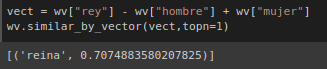
\includegraphics[width=0.6\textwidth]{Graphics/word2vec.png}
%    \caption{Grado de aprendizaje de la semántica de Word2Vec en español}
%    \label{fig:word2vec}
%\end{figure}
%

\subsection{difflib}
Este módulo de Python proporciona clases y funciones para comparar secuencias. Se puede usar, por ejemplo, para comparar archivos y puede producir información sobre diferencias de archivos en varios formatos, incluidos HTML y contexto y diferencias unificadas.

 \subsubsection{clase SequenceMatcher}
 Esta es una clase flexible para comparar pares de secuencias de cualquier tipo, siempre que los elementos de la secuencia se puedan modificar. El algoritmo básico es anterior a un algoritmo publicado a fines de la década de 1980 por Ratcliff y Obershelp con el nombre hiperbólico de ''coincidencia de patrones gestálticos'', y es un poco más elegante. La idea es encontrar la subsecuencia coincidente contigua más larga que no contenga elementos ''basura''; estos elementos ''basura'' son los que no son interesantes en algún sentido, como líneas en blanco o espacios en blanco. (El manejo de basura es una extensión del algoritmo de Ratcliff y Obershelp). Luego, la misma idea se aplica recursivamente a las partes de las secuencias a la izquierda y a la derecha de la subsecuencia coincidente. Esto no produce secuencias de edición mínimas, pero tiende a generar coincidencias que ''parecen correctas'' para las personas.
 \subsubsection{get$\_{}$close$\_{}$matches}
 Método para seleccionar la secuencia más similar a una secuencia dada dentro de un vocabulario.

\subsection{Boto3}
Se utiliza el Kit de desarrollador de software (SDK por sus siglas en inglés) de AWS para Python (Boto3) para crear, configurar y administrar servicios de AWS, como Amazon Elastic Compute Cloud (Amazon EC2) y Amazon Simple Storage Service (Amazon S3). El SDK proporciona una API orientada a objetos, así como acceso de bajo nivel a los servicios de AWS.

Este SDK es empleado para acceder a los datos.

\subsection{pathlib}
Este es un módulo de Python que ofrece clases que representan rutas de sistemas de archivos con semántica apropiada para diferentes sistemas operativos. Las clases de ruta se dividen entre rutas puras, que proporcionan operaciones puramente computacionales sin Entrada/Salida (I/O por sus siglas en inglés), y rutas concretas, que heredan de rutas puras pero también proporcionan operaciones de I/O.

La clase Path de esta biblioteca es ampliamente usada en este trabajo.

\section{Implementación de un prototipo}
El prototipo implementado realiza todos los pasos mencionados en la sección \ref{section:proposal:stepbystep}

Primeramente se realizó todo el trabajo en Google Colaboratory (Colab para abreviar).

\subsection{Extracción de los Datos}
Para la extracción de los datos se utilizó la biblioteca boto3 con acceso al almacenamiento en la nube donde se encontraban los datos.
Para ello se importa el método client de boto3, el cual es instanciado en la url donde se encuentra el conjunto de datos, además de las claves de acceso, las cuales por privacidad del dueño de las mismas se sustituyen por valores de "X". 

\vspace{0.5cm}

\begin{lstlisting}[language=Python, caption={Instanciar cliente s3}, label={code:s3client}]
from boto3 import client

s3_client = client(
    "s3",
    config=Config(
        signature_version="s3v4",
        retries={"max_attempts": 10},
        s3={"addressing_style": "path"},
    ),
    region_name="ams3",
    endpoint_url="https://ams3.digitaloceanspaces.com",
    aws_access_key_id="XXXXXXXXXXXXXXXX",
    aws_secret_access_key="XXXXXXXXXXXXXXXXXXXXXXXXXXXXX",
)
\end{lstlisting}

Una vez obtenido el cliente configurado se descargan los datos del mismo, conociendóse que se encuentran en el bucket "lsc-corpus", los de las señas aisladas, puesto que son los únicos datos con seguridad de la seña que corresponde a cada frase.

\vspace{0.5cm}

\begin{lstlisting}[language=Python, caption={Descargar usando el cliente s3}, label={code:download_s3client}]
from pathlib import Path

root=Path("/content")
bucket="lsc-corpus"    

paginator = s3_client.get_paginator('list_objects_v2')
pages = paginator.paginate(Bucket=bucket)

for page in pages:
    for obj in page['Contents']:
        extension = obj['Key'].split('.')[-1]
        name=obj['Key'].split('.')[0]
        if extension  in ['json']:
		  drivepath=(root/f"tesis-generacion-lsc/{obj['Key']}").resolve()
  		  (drivepath/'..').resolve().mkdir(parents=True,exist_ok=True)
  		  drivepath.touch()
  		  s3_client.download_file(bucket,obj['Key'],str(drivepath))
  
\end{lstlisting}
Aquí se realiza un paginado para poder recorrer de manera adecuada  los elementos del bucket para luego chequear la extensión de los archivos contenidos en cada página.
Se conocen previamente que los datos anotados de los puntos de interés estaban recogidos en archivos con extensión json por cada frase. En la primera parte del código se importa la clase Path de pathlib para trabajar de manera rápida y efectiva con los directorios que se van creando.

\subsection{Limpieza de los datos}
Una vez ya se posean los archivos json referentes a cada frase del corpus se pueden entonces cargarlos para limpiarlos y organizarlos en un dataset mejor estructurado donde estén todas las frases juntas.

En este código utilizamos expresiones regulares para la limpieza de las llaves, ya que incurrían en faltas de ortografía, errores tipográficos y de copiado.
La primera expresión elimina todo lo que esté entre paréntesis en las llaves, puesto que esto no aporta nada a la información semántica de los mismos. Luego se reemplaza todas las ''nn'' por una ''ñ'' 
y se eliminan los dígitos que hayan quedado de manera residual del primer método.Para a modo de cierre de la limpieza de las llaves eliminar todos los guiones entre palabras para que esten de manera individual.
\vspace{0.5cm}

\begin{lstlisting}[language=Python, caption={Cargar los json y limpiar las llaves}, label={code:load_and_clean}]

import numpy as np
import json
import re

root_tesis = (root/f"tesis-generacion-lsc/").resolve()
cendsor_path = "cendsor-corpus/keypoints/"
fps=24

word_poses_dict={}

for dirpath,dirnames,filenames in os.walk(root_tesis/cendsor_path):
  for filename in filenames:
    key,extension=filename.split('.')
	
	###########################
	# Limpieza de las llaves
	###########################
	
    key=re.sub(r"\s*\(.*\)","",key)
    key= key.replace("nn",'ñ')
    key=re.sub(r"\s?\d","",key)
    key = key.replace("-"," ") 
    
	###########################
	
    with open((root_tesis/cendsor_path/filename).resolve(), 'r', encoding='utf-8') as json_list:
      poseframes=np.array(json.load(json_list))
      json_list.close()
		
	  #######################################################
	  # Limpieza y reajuste de los frames de los gestos
	  #######################################################
      filtro = [m!=0.0 for m in  np.mean(poseframes, axis=1)]
      
      poseframes=poseframes[filtro]

      total_frames = poseframes.shape[0]

      n = math.floor(total_frames/fps)

      poseframes= poseframes[::n,:]

      while poseframes.shape[0]>24:
        if poseframes.shape[0]%2:
          poseframes=poseframes[1:,:]
        else:
           poseframes=poseframes[:-1,:]
	  #########################################################
	  
      single_gesture = poseframes.tolist()
      try:
        word_poses_dict[key].append(single_gesture)
      except:
        word_poses_dict[key]=[single_gesture]
        
\end{lstlisting}
En el caso de los gestos existen en el corpus frames en los cuales los modelos no detectaban nada y por tanto estos devolvían (0,0,0) para todos los puntos de interés de ese frame. Por tanto se hace uso de la biblioteca json para cargar el archivo y de la biblioteca numpy para realizar la limpieza de una manera más cómoda y rápida.
Luego de obtener la máscara (filtro) con la información de los frames vacíos, simplemente se indexa en el arreglo numpy guardando su resultado como si fuera ahora el arreglo original.
Pero proseguía un problema más, el tamaño de los frames no era parejo. Algunos archivos tenían más frames que otros, por lo tanto se decidió llevarlos todos a 24 frames utilizando la función floor de la biblioteca math para obtener un valor que al dividir por la cantidad de frames no diera superior y fuera entero.
Posteriormente, como no van a quedar exactamente de tamaño 24, sino mayor, se va reduciendo en 1 la cantidad de frames por los extremos hasta llegar a la cantidad deseada.

Como información adicional se guarda el diccionario tanto en la nube como en local para su mejor aprovechamiento y eliminarnos pasos extras a la hora de probar el modelo.

%\subsection{Cargando el embedding de palabra}
%Primeramente se debe descargar el archivo de los KeyedVectors el cual pesa alrededor de los 3Gb, razón por la cual se ha estado desarrollando todo este flujo de trabajo directamente en Colab puesto que es un gran modelo para capturar significado semántico dado lo limitado del corpus en ese sentido.
%\vspace{0.5cm}
%
%\begin{lstlisting}[language=Bash, caption={Descargar datos del modelo KeyedVectors de su sitio web}] 
%  
%  $ wget "https://zenodo.org/record/1410403/files/keyed_vectors.zip" 
%  $ unzip keyed_vectors.zip
%  
%\end{lstlisting}
%
%Luego de descargado y descomprimido se puede entonces cargar el modelo.
%
%\begin{lstlisting}[language=Python, caption={Cargar modelo de KeyedVectors}]
%  from gensim.models import KeyedVectors
%  wv = KeyedVectors.load('complete.kv', mmap='r')
%\end{lstlisting}
%Como se aprecia, KeyedVectors es un modelo perteneciente a la biblioteca gensim, el cual es uno de los elementos que componen a Word2Vec y justamente el único que necesitamos para nuestro propósito de  capturar la semántica de las frases. Cargar completamente el modelo Word2Vec exige mucha memoria RAM puesto que es un modelo de más de 7 Gb en su completitud y es esa la razón por la que se escoge solamente el diccionario de los vectores claves (KeyedVectors).
%
%.El archivo complete.kv es el resultado de descomprimir el modelo descargado.
\subsection{Encontrando similitud de palabras}
Como se plantea en la propuesta primeramente se debe asegurar de que se logre encontrar una palabra dentro del vocabulario de nuestro embedding, por eso se declara el siguiente método a continuación.

\begin{lstlisting}[language=Python, caption={Método para encontrar palabras similares en un vocabulario}]
  def find_similar(word, vocab):
  	import difflib
  	best_match=difflib.get_close_matches(word,vocab)
  	if len(best_match) != 0:
    	score = difflib.SequenceMatcher(None,word,best_match[0]).ratio()
    	return best_match[0],score
    else:
    	return None
    	
\end{lstlisting}
En este método se utiliza el método get$\_{}$close$\_{}$matches para encontrar la palabra más parecida sintácticamente a la proporcionada, en el vocabulario dado.
Luego si encuentra que existe alguna palabra que sea similar, pues se instancia una clase SequenceMatcher para hallar que tan similares son. Por supuesto este ultimo paso solo es necesario en caso de necesitarse cuantificar la similitud.

%\subsection{Extrayendo la matriz de cada frase}
%El siguiente método genera una matriz de $num\_{}vecs$ x $vec\_{}dim$ que es la dimensión de los vectores. 
%Primero se crea un diccionario de palabras mal escritas (posible en este escenario dado que solo se cuentan con poco más de 1050 vocablos) y además para no arrastrar el error semántico de unos datos erróneos se escogen palabras de igual significado semántico.
%
%Luego se crea un arreglo numpy de ceros con las dimensiones específicadas para posteriormente conformarlo con los vectores de cada palabra de la frase de 5 vocablos en el caso del corpus utilizado.
%
%\begin{lstlisting}[language=Python, caption={Obtener el vector dada una palabra}]
%  def get_vector(key,word_vectors,num_vecs=5):
%  wrong_words={'antonimo': 'antónimo',
%              'audiologia':'audiología',
%              'barsura':'basura',
%              'defectologia':'defectología',
%              'empanizar':'empanar',
%              'insipido': 'insípido',
%              'investar':'inventar',
%              'lexicologia': 'lexicología',
%              'ostion':'ostra',
%              'panciencia':'paciencia',
%              'policlinica': 'policlínica',
%              'querologia':'querología',
%              'rehablilitacion':'rehabilitación',
%              'sacapunta':'sacapuntas',
%              'señacionario':'diccionario',
%              'señario':'libro', 
%              'zapia':'compartición'}
%  vector=np.zeros((num_vecs,word_vectors.vector_size))
%  
%  for i,word in enumerate(key.split(" ")):
%    if word in word_vectors.vocab.keys():
%
%      wordvec = word_vectors[word]
%    else:
%      word=wrong_words[word]
%      nword, similarity = find_similar(word,word_vectors.vocab.keys())
%      print(key,"Not Founded")
%      print(nword,similarity)
%
%      wordvec = word_vectors[nword]
%    vector[i:]=wordvec
%  return vector
%\end{lstlisting}
%Luego de creado el arreglo de numpy, se verifica que la palabra esté en el vocabulario del embedding antes de indexar la palabra en busca de su vector. En caso de no existir la palabra pues se utiliza el método descrito en la subsección anterior para hallar un vocablo sintácticamente similar que si pertenezca al vocabulario del embedding.
%
%Finalmente, después de rellenado el arreglo de numpy, este es retornado.

%\subsection{Creando los conjuntos}
%
%En este código creamos y llenamos los conjuntos $X$ e $y$ para su ulterior uso en el modelo. $num\_{}vecs$ es escogido como el mayor número de palabras de todo el conjunto de datos, el cual en exploraciones a los datos fue revelado que es 5.
%
%\begin{lstlisting}[language=Python, caption={Crear los conjuntos X e y}]
%  
%X=[]
%y=[]
%
%num_vecs=max([len(key.split(" ")) for key in dataset.keys()])
%
%for key,gestures in dataset.items():
%  vector=get_vector(key,word_vectors,num_vecs)
%  X.append(vector)
%  y.append(np.array(gestures[0]).reshape((fps,sum([dim[0] for dim in dims]),dims[0][1]))) 
%\end{lstlisting}
%Para evitar el problema de que a cada frase le correspondieran varias señas, con alta probabilidad de que fueran distintas, se optó por solamente escoger la primera de las señas como representativa de las demás.

\subsection{Métodos para la animación}
Primero instanciamos los valores necesarios para animar correctamente un conjunto de puntos con estructura igual a la de los datos .

\begin{lstlisting}[language=Python, caption={Instanciar datos necesarios para animar }]
body_dim = 25*3
left_dim = 21*3
right_dim = 21*3

dims=[(25,3),(21,3),(21,3)]

bodyjoints=[[1,7],[4,8],[9,10],[11,12],[11,13],
[12,14],[11,23],[12,24],[23,24],[13,15],[14,16]]
leftjoints=[[0,1],[1,2],[2,3],[3,4],
            [0,5],[5,6],[6,7],[7,8],
            [5,9],[9,10],[10,11],[11,12],
            [9,13],[13,14],[14,15],[15,16],
            [13,17],[17,18],[18,19],[19,20],[0,17]]
rightjoints=leftjoints

fullbodyjoints=[bodyjoints,leftjoints,rightjoints]

parts_names=["body","left","right"]
\end{lstlisting}

Utilizamos el siguiente método en caso de que los puntos no vengan en formato (24,67,3) y simplemente vengan en formato (24,201)

\begin{lstlisting}[language=Python, caption={Extraer las partes en 3d }]
def extract_3d_shape(array,dims):
      init=0
      ending=0
      parts=[]
      for dim in dims:
        ending+=dim[0]*dim[1]
        parts.append(array[:,init:ending].reshape((array.shape[0],dim[0],dim[1])))
        init+=dim[0]*dim[1]

      single_gesture={parts_names[i]:parts[i] for i in range(len(dims))}

      return single_gesture
\end{lstlisting}

Utilizamos la lista con las dimensiones para de poder, en caso de ser necesario, incluir graficaciones de otras partes del cuerpo que fueron excluidas.

El siguiente método contituye la base de todos los métodos para las animaciones de este trabajo.
Se utilizan varias clases y métodos de la biblioteca matplotlib para realizar la animación.

FuncAnimation recibe la figura en la que trabajar,la función de actualización, que es la encargada de la transición entre frames, y por último la cantidad de frames a animar.

\begin{lstlisting}[language=Python, caption={Método base para animar }]
import matplotlib.pyplot as plt
from matplotlib.animation import FuncAnimation
from matplotlib import rc
import matplotlib.cm as cm

def transform_data(Data,i):
    from scipy.spatial.transform import Rotation as R

    r = R.from_rotvec(np.pi/2 * np.array([0,0,1]))

    X=np.array(Data[i,:,0])
    Y=np.array(-Data[i,:,1])
    Z=np.array(Data[i,:,2])
    meanpoint=(X[X!=0].mean(),Y[Y!=0].mean(),Z[Z!=0].mean())

    D = np.array([x if x!=(0.0,0.0,0.0) 
                    else meanpoint
              for x in zip(X, Y, Z) ])
    D = r.apply(D)
    return D

def animate(
			Data,
			frames=None,
			figsize=(7.0,3.5),
			elev=None,
			angle=None,
			dims=dims,
			text=False,
			joints=False):
			
  rc('animation',html='jshtml')
  fig_size_x,fig_size_y=figsize

  plt.rcParams["figure.figsize"]= [fig_size_x,fig_size_y]
  plt.rcParams['figure.autolayout']= True

  fig = plt.figure()
  ax = fig.add_subplot(projection='3d')
  colors=['b','y','r','k']
  
  def update(i):
    ax.clear()

	D = transform_data(Data,i)	
	
    s=0
    e=0
    for j, dim in enumerate(dims):
      dim = dim[0]
      e+=dim

      x=D[s:e,0]
      y=D[s:e,1]
      z=D[s:e,2]

      # print((x.mean(),y.mean(),z.mean()) != meanpoint )
      if (x.mean(),y.mean(),z.mean()) != meanpoint:
        # print(x.mean(),y.mean(),z.mean())
        ax.plot(D[s:e,0],D[s:e,1],D[s:e,2],f'{colors[j]}.')
      if text:
        for p in range(s,e):
          ax.text3D(D[p,0],D[p,1],D[p,2],str(p))
      if joints:
        for h,k in fullbodyjoints[j]:
          ax.plot([D[s+h,0],D[s+k,0]],[D[s+h,1],D[s+k,1]],[D[s+h,2],D[s+k,2]],f'{colors[j]}')
      s+=dim

    ax.set_axis_off()
    if elev and angle:
      ax.view_init(elev,angle) 

    
    return ax

  if frames is None:
    frames=24
  return FuncAnimation(fig,update,frames=frames,repeat=True)
\end{lstlisting}

Se utiliza la clase Rotation del módulo transform de scipy para rotar de manera efectiva la figura para que sea visualmente atractiva la animación desde una vista frontal. Al igual que si existen muchos puntos espaciales en el (0,0,0) se halla la media de los puntos distintos del cero del espacio para no distorsionar el graficado de la animación, esto ocurre por fallos del método que creó el corpus inicialemente al no detectar alguna región del cuerpo, es decir ya los datos con los que se cuentan vienen dados con cierto grado de error.
Luego, para que sea visualmente llamativo, se utilizan las dimensiones de las distintas partes del cuerpo para graficar de un color diferente cada una de las partes y se utilizan las uniones declaradas inicialmente. 

En caso de ser necesario puede agregarse el texto del número correspondiente al punto para mejor visualización.

También se incorpora la posibilidad de modificar las dimensiones de la figura, así como el angl¡ulo de azimut y de elevación correspondiente.


En cuanto al último método, este solo representa una composición de los métodos anteriores con una organización intermedia de los arreglos correspondientes a cada parte en caso de que la entrada no tenga la estructura idónea para la graficación.

\begin{lstlisting}[language=Python, caption={Graficar la animación }]
  
def plotanimation(result):
	if result.shape[2]==201:
  		dict_parts=extract_3d_shape(result[0],dims)
      
  		body_frames = dict_parts["body"]
  		left_frames = dict_parts["left"]
  		right_frames = dict_parts["right"]

  		result = np.hstack((body_frames,left_frames,right_frames))
  		

  a=animate(result,result.shape[0],(12,10),90,1,dims,text=False,joints=True)
  
  return a
\end{lstlisting}

%\section{Entrenamiento}
%El modelo presentado, como se mencionó en capítulos anteriores, necesita ser debidamente entrenado. Dado que el dominio e imagen del conjunto disponible para el entrenamiento es alarmantemente corto en comparación con los vocablos utilizados comúnmente en el día a día por una persona promedio. Hablamos de que alrededor de 20 mil vocablos son empleados a diario en una jornada normal, mientras que el corpus brindado por el CENDSOR solo cuenta con poco más de 1050 vocablos(con algunos teniendo más de 1 respresentación visual diferente)
%
%Con estas condiciones del corpus, el enfoque adoptado para el entrenamiento es el de generar sobreadecuación (overfitting) sobre los únicos vocablos conocidos para que así al componerse con el uso del embedding de palabra puedan encontrarse similaridades semánticas entre una palabra desconocida y una del vocabulario disponible.
%subsection{Definición del modelo}
%
%Como se explicó en la propuesta, el enfoque adoptado para este modelo es el de utilizar redes neuronales recurrentes, más específicamente LSTM multicapas con capas deconvolucionales para ampliar las dimensiones.
%\begin{lstlisting}[language=Python, caption={Diseño del modelo}]
%
%from tensorflow.keras.layers import InputLayer, LSTM , Conv1DTranspose, Reshape
%from tensorflow.keras.models import Sequential
%from tensorflow_addons.metrics.r_square import RSquare
%
%def get_model(X, y):
%    model = Sequential()
%    model.add(InputLayer(X.shape[1:]))
%    model.add(LSTM(128, return_sequences=True, activation="relu"))
%    model.add(LSTM(256, return_sequences=True, activation="relu"))
%    model.add(Conv1DTranspose(filters=100,kernel_size=10))
%    model.add(LSTM(128, return_sequences=True, activation="relu"))
%    model.add(Conv1DTranspose(filters=150,kernel_size=11))
%    model.add(LSTM(201,return_sequences=True))
%    model.add(Reshape(y.shape[1:]))
%    loss = "mae"
%    metrics = RSquare()
%    model.compile(optimizer='Adam', loss=loss, metrics=metrics)
%    return model
%\end{lstlisting}
%
%Las cantidad de unidades fueron escogidas basándonos en la unidades que reportaron beneficios para el trabajo precedente a este [\cite{leynier-lsc-2021}].
%Para la función de pérdida fue seleccionado el Error Medio Absoluto(MAE por sus siglas en inglés) puesto que compara efectivamente la diferencia de posición espacial dados los datos con que se cuentan.
%Además se usa el R Cuadrado como métrica de puntuación para poder entrenar de manera efectiva.
%
%
%Las opciones basadas en transformadores requerían de cantidades de datos superiores a las que se contaban así que se tomó solo en cuenta los estudios referentes a las Redes neuronales recurrentes LSTM.
%
%
%Se utilizó un método supervisado de entrenamiento usando un enfoque regresivo dada la no existencia de categorías calaramente definidas en el espacio de todas las posibles señas.
%\begin{lstlisting}[language=Python, caption={Graficar la animación }]
%
%
%from tensorflow.keras.callbacks import EarlyStopping, ModelCheckpoint
%from sklearn.model_selection import KFold,cross_val_score
%
%X,y=(np.array(X),np.array(y))
%X_train,X_test,y_train,y_test = train_test_split(X,y,test_size=0.3,random_state=42)
%
%checkpoint_path= (droot_tesis/"generacion-lsc_0001.ckpt").resolve()
%
%num_folds=5
%batch_size=32
%epochs=1000
%
%kfold = KFold(n_splits=num_folds, shuffle=True)
%
%# K-fold Cross Validation model evaluation
%acc_per_fold=[]
%loss_per_fold=[]
%fold_no = 1
%for train, val in kfold.split(X, y):
%
%  model = get_model(X, y)
%  if checkpoint_path.exists():
%    model.load_weights(checkpoint_path)
%
%  ckpt_callback= ModelCheckpoint(
%      filepath=str(checkpoint_path).format(epoch=0),
%      save_weights_only=True,
%      verbose=1,
%      save_freq=5*batch_size)
%  
%  callback = EarlyStopping(
%      monitor= "loss",
%      patience=10)
%  
%  print(model.summary())
%  # Generate a print
%  print('--------------------')
%  print(f'Training for fold {fold_no} ...')
%
%  # Fit data to model
%  history = model.fit(
%      X[train],
%       y[train],
%       batch_size=batch_size,
%       epochs=epochs,
%       callbacks=[callback,ckpt_callback])
%
%  # Generate generalization metrics
%  scores = model.evaluate(X[val], y[val],)
%  print(f'Score for fold {fold_no}: {model.metrics_names[0]} of {scores[0]}; {model.metrics_names[1]} of {scores[1]*100}%')
%  acc_per_fold.append(scores[1] * 100)
%  loss_per_fold.append(scores[0])
%
%  # Increase fold number
%  fold_no = fold_no + 1
%
%\end{lstlisting}
%
%Se utiliza un entrenamiento con Kfold para iterar por conjuntos de datos separados de forma aleatoria y así lograr evaluar para todos los valores además de 1000 epochs.
%Se utilizan callbacks de parada temprana para en caso de que los valores de las funciones de puntuación y de pérdida no varían mucho luego de un cierto tiempo y además se usa un callback para salvar los pesos del modelo durante el entrenamiento en caso de colapso del servicio de Colab o de fallos eléctricos. 
%Dicha salva de los pesos del modelo es retomada en cada iteración del método Kfold para garantizar que se haga overfitting sobre los datos.
%
%Podrá parecer extraño que se quiera sobreadecuar el modelo al conjunto de datos pero no es la primera vez que se hace esto sobre el vocabulario disponible de cierta tarea o problema, como se hizo en el caso de GPT3, el cual sobreadecúa los datos de todo internet logrando así dominar el vocabulario dado.

\subsection{Experimentos}
%Como desenlace del entrenamiento del modelo se logró evidenciar buenos resultados dada la simpleza del método presentado, las limitantes y problemáticas del conjunto de datos.
%
%\begin{figure}[ht!]
%    \centering
%    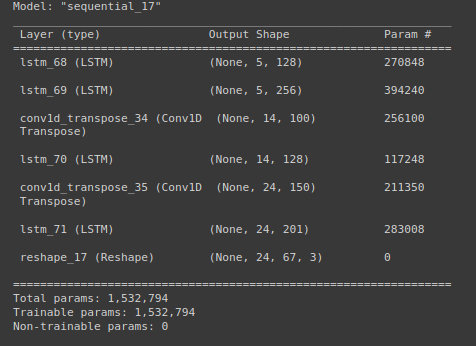
\includegraphics[width=0.8\textwidth]{Graphics/resumen_modelo.png}
%    \caption{Resumen de las capas y parametros del modelo}
%    \label{fig:resumen_modelo}
%\end{figure}
%
%Durante el entrenamiento se utilizaron las métricas Error Promedio Absoluto (MAE por sus siglas en inglés) como función de pérdida y R Cuadrado (R Squared) como función de puntuación dado que este es un problema de regresión.
%
%
%\begin{figure}[ht!]
%    \centering
%    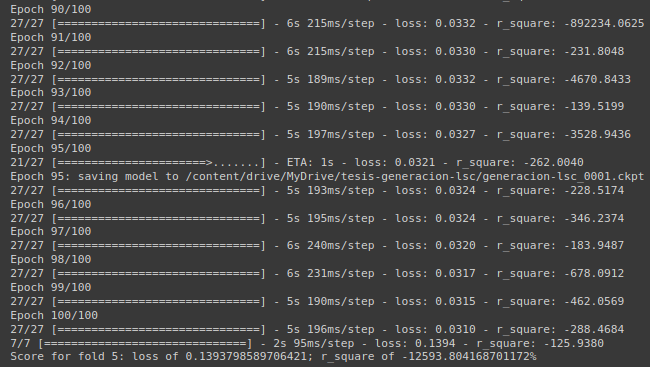
\includegraphics[width=0.8\textwidth]{Graphics/metricas_last_epochs.png}
%    \caption{Resultado de las métricas de los últimos epochs del modelo durante el entrenamiento}
%    \label{fig:metricas_last_epochs}
%\end{figure}
%
%Aquí se puede presenciar una comparativa de los resultados obtenidos para la primera frases del conjunto de datos.
%
%\begin{figure}[ht!]
%    \centering
%    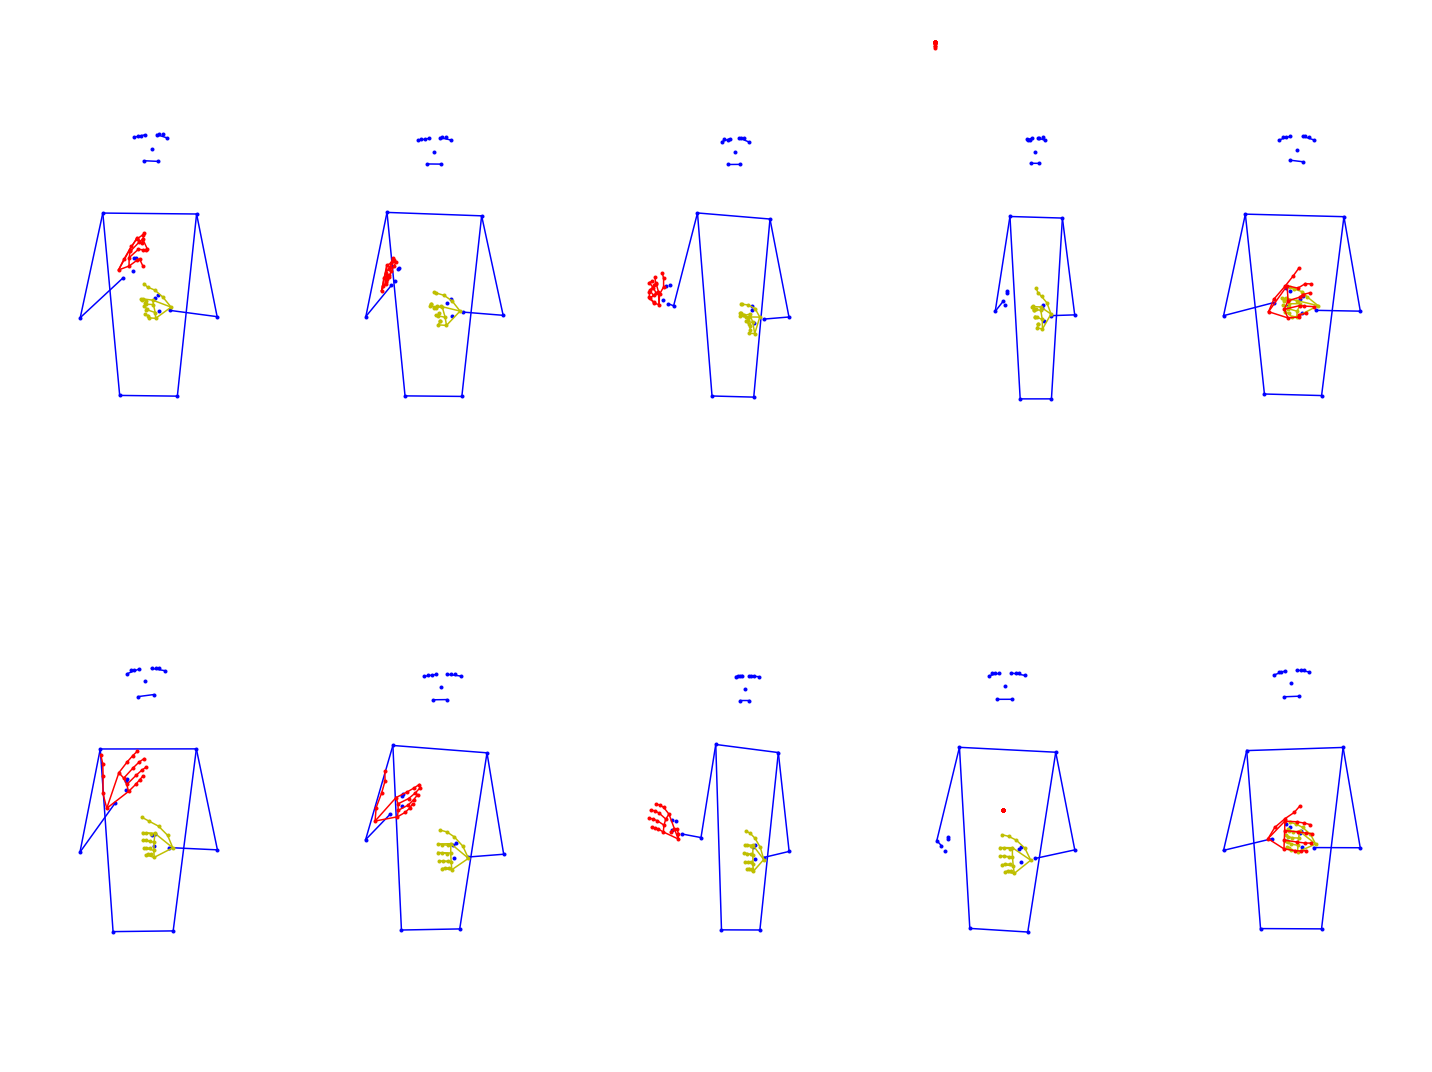
\includegraphics[width=0.8\textwidth]{Graphics/abandonar_comparison.png}
%    \caption{Comparativa de la frase ''abandonar'' . Fila superior los valores predichos. Fila inferior los valores reales}
%    \label{fig:abandonar_comparison}
%\end{figure}
%
%\begin{figure}[ht!]
%    \centering
%    \includegraphics[width=0.8\textwidth]{Graphics/por_la_mañana_comparison.png}
%    \caption{Comparativa de la frase ''por la mañana'' . Fila superior los valores predichos. Fila inferior los valores reales}
%    \label{fig:mannana_comparison}
%\end{figure}

\subsection{Discusión}
%Visualmente se obtuvieron buenos resultados, pero sin una medida específica salvo la percepción del autor.
%Muchos de los puntos referentes a los dedos no se detectaron como se correspondía y no se tuvo una métrica que describiera bien la puntuación del modelo de regresión.
% Esto se debe en gran parte a que los datos con que se contaban presentaban errores y, al ser pocos, se transmitían de manera fácil al modelo durante el entrenamiento, a pesar de emplear la sobreadecuación del mismo al corpus brindado.
%
%A pesar de ello se obtuvieron resultados bastante aceptables y una puntuación del R Cuadrado bastante cercana al máximo posible que es 1.

\backmatter

\begin{conclusions}

%%%%%%%%%%%%%%%%%%%%%
% Ajustarlas a los resultados obtenidos
%%%%%%%%%%%%%%%%%%%%%

  La generación de avatares para la Lengua de Señas Cubana representa el principal objetivo del trabajo. Durante la investigación se generan nuevos métodos, estructuras y corpus que posibilitan una mejor comprensión de esta temática.
   Se introduce la problemática presente en el contexto social correspondiente y se profundiza en el estado del arte de diversos campos como la escritura de señas, haciendo énfasis en su estructura y composición, reconocimiento de señas, tecnología de avatares, modelos generativos y  interpolación de movimiento, detectándose un crecimiento de la aceptación de los modelos que utilizan inteligencia artificial y  aprendizaje de máquina, además de, indagar acerca de los únicos trabajos encontrados que tratan la Lengua de Señas Cubana.
   Se identificaron los distintos rasgos, acciones y señas encontrados pertenecientes a la Lengua de Señas Cubana gracias a los trabajos previamente efectuados sobre el tema.
   Se propuso una estructura de métodos y clases para la correcta interpolación y adición de una secuencia de señas, lográndose así una correcta generación de movimientos suaves y definidos del esqueleto del avatar. Esta propuesta para la generación de avatares para la Lengua de Señas Cubana, utilizando el corpus generado por anteriores investigaciones, fue concretada en un prototipo de clases que utilizan interpolación e integración numérica para resolver los problemas presentados.
 	Se obtuvo un avatar que consigue ejecutar de manera armónica los movimientos asociados a cada token de seña incluyendo cualquier combinación de los mismos sin importar cuán extensa sea. Además se proporcionaron pautas para el uso y mejoramiento de la bases de datos de las señas cubanas actualmente disponible.

\end{conclusions}

\begin{recomendations}

%%%%%%%%%%%%%%%%%%%
% Retocarlas y ajustarlas un poco al tema
% Recomendar la continuacion de la investigacion
% Para la generacion de avatars humanos
%%%%%%%%%%%%%%%%%%%
Con este trabajo se ayuda a una nueva rama de investigación y desarrollo referente a la lengua de señas cubana, ya que forma un pilar esencial en cualquier sistema de traducción de lenguas de señas. Al ser este un trabajo novedoso en el campo de la generación de avatares señantes, se deja como pauta inicial para futuros trabajos y una guía del proceder ante los limitados datos disponibles.

Se sugiere:
\begin{itemize}
\item Estudiar la generación de archivos de captura de movimiento como BVH  y el cálculo de los vectores de rotación de brazos, manos y dedos.
\item Lograr transformar un vídeo de un avatar animado en una persona real haciendo uso de los modelos generativos, en especial el uso de los métodos de imagen a imagen (img2img)
\item Desarrollar alternativas con el uso de otros modelos generativos de imágenes para la humanización del avatar presentado.
\end{itemize}
 Se recomienda, a los investigadores de Cuba, lingüistas y especialistas de la lengua de señas y a toda la comunidad:
 \begin{itemize}
 \item Crear conciencia sobre la importancia y necesidad de este tipo de estudios y herramientas para el correcto desarrollo de la comunidad sordo-muda cubana
 \item Trabajar unánimemente en pos de lograr un corpus correctamente anotado y tanto extenso, como generalizado, para así obtener una herramienta de utilidad para que, en manos de los hipoacúsicos, sea la llave para romper las barreras comunicativas que les impiden desenvolverse y desarrollarse en nuestro país actualmente. 
\end{itemize}  
\end{recomendations}

\printbibliography[heading=bibintoc]

\end{document}